

\chapter{Evaluation and Benchmarking}


To finally assess the strength of the approach explained in the previous chapters, the resulting implementation has to be benchmarked. To do this, the agent played against a variety of other programs, as well as against a human poker player. The results are outlined in the following chapter.
 

\section{Benchmark Tournament}

To estimate the strength of my implementation, I ran an extensive round-robin tournament with all the bots mentioned. Each match consists of an ordinary heads-up match of 3000 hands between two players. The cards played are recorded (or the seed used to shuffle is saved) and then the players' memories are reset, they switch positions and play a second 3000 hands with the switched cards. The purpose of the duplicate match is to reduce the variance of the outcome. In total, each opponent plays 6 such duplicate matches against each other, resulting in 36000 hands (18'000 unique hands) played for each outcome. During the course of the whole tournament, 540'000 hands were played, which took approximately three weeks to fully compute.

\subsection{Rules}
For the tournement, the same game rules were used, as in the Computer Poker Competition 2009, held at the International Joint Conferences on Artificial Intelligence in Passadena, CA.

The Tournament is played in a special veriant of no-limit called Doyle's Game: in this variant the stack sizes of both players are reset after every hand, and the score is kept separately. This is akin to both players buying in for 200 big blinds every hand, cashing in their chips at the end of the hand, and buying in for 200 big blinds again the next hand. The exact rules, as stated on the homepage of the competition (see \cite{Hawkin2009}):

\begin{itemize}
	\item Each hand is a hand of reverse blinds no-limit texas hold-em. This means that the second player (the dealer) puts in the small blind, and the first player puts in the big blind (2 small blinds). Counterintuitively, this means that the second player (dealer) has the first action on the preflop betting round (the first betting round), while the player off the button has first action in the later stages.
	\item The blinds are 1\$/2\$ no limit with stacks of 200 big blinds, meaning that the small blind is 1 chip, the big blinds is 2 chips and both players start each hand with 400 chips.
	\item The maximum bet size is that which brings the total number of chips a player has put into the pot to 400. The nominal minimum bet size is either 2 chips at the beginning of a round or the size of the most recent bet. If the nominal minimal bet is larger than the maximum bet, then the minimum bet is equal to the maximum bet. Raises must be of an integer number of chips. 
	\item There is no limit to the number of raises that can be made.
	\item In this competition, there is no mucking: all players will reveal their cards at every showdown. Folded cards though are never shown.
	\item Any illegal action is interpreted as a call if raise is illegal. If it is a raise for an illegal amount, it is interpreted as the closest possible raise amount.
\end{itemize}

\subsection{Benchmark Opponents}

The field of contenders consists of both pure dummy bots, as well as commercial bots found in the \textit{Poker Academy} Software. Unfortunately, the bots out of \textit{Poker Academy} were protected, and had some relentless (though legal) reverse-engineering had to be applied to be able to use them outside of \textit{Poker Academy}. \cite{Andersson2006} also used some of these bots for his benchmarks, but as he didn't extract them for usage on the pokerserver software of the \textit{Annual Computer Poker Competition}, he required much more hands, as  \textit{Poker Academy} doesn't allow reverse matches or repetition of the same cards between different opponents.

\subsubsection{Dummies}
The first two very simple bots, either always called, or always raised. If checking was legal, they both checked.

\subsubsection{JamBot}
JamBot is part of  \textit{Poker Academy} and employs a simple push-or-fold strategy devised by David Sklansky. Such strategies of either fold or go all-in are usually only played when the stack of a player in a tournament becomes to small to allow playing multiple stages. 
\subsubsection{AveryBot}
This bot is based on the Averybot engine from \textit{Poker Academy}. It uses basic opponent modeling and is described as playing an aggressive strategy meant for No-Limit tournaments. The basic strategy was reportedly inspired by the writings of poker author T.J. Cloutier.


\subsubsection{XenBot}
XenBot is an agent programmed by the University of Alberta Computer Poker Research Group. It was featured in the computer game \textit{Stacked} and is also part of \textit{Poker Academy}. While not state of the art anymore, it's skill is often compared with that of a beginner to intermediate poker player. The basic strategy follows \cite{Billings1995}.
 

\subsection{Results} 
\begin{table}
\begin{center}
  \begin{tabular}{ l|c c c c c c|c}

& A. Call& A. Fold& AveryBot& JamBot& UZHoldem& XenBot& avg. \\
 \hline
Always Call &  - & 0.255 & -6.334 & -12.258 & -20.527 & 0.697 & -6.361 \\ 
Always Fold & -0.255 &  - & -0.502 & -0.044 & -0.596 & -0.750 & -0.358 \\ 
AveryBot & 6.334 & 0.502 &  - & 0.410 & -1.592 & 0.2753 & 0.988 \\ 
JamBot & 12.258 & 0.044 & -0.410 &  - & -0.003 & -0.817 & 1.845 \\ 
UZHoldem & 20.527 & 0.596 & 1.592 & 0.003 &  - & -0.752 & 3.661 \\ 
XenBot & -0.697 & 0.750 & -0.2753 & 0.817 & 0.752 &  - & 0.225 \\ 

 \end{tabular}
\end{center}
 
\caption{Benchmark tournament results}

\end{table}

As we can see, UZHoldem plays reasonably strong against most opponents and wins by a huge margin against the dummy bots. A few limitations though apply: All the bots out of the \textit{Poker Academy} software are bots also capable at playing ring table games. They are no heads-up specialist and probably more targeted to the more popular variations of the game with 4 and more players. 

Figure \ref{fig:result-averybot} to \ref{fig:result-alwayscall} show the aggregated graphs (average of all matches played against a specific opponent) of UZHoldem versus his opponents  \footnote{The scripts to create these graphs can be found in the \texttt{uzholdem.util.matchanalytics} package in the accompanied source code. To run them, a proper installation of the \textit{R} environment for statistical computing is required}: 


\begin{figure}[!ht]
\centering
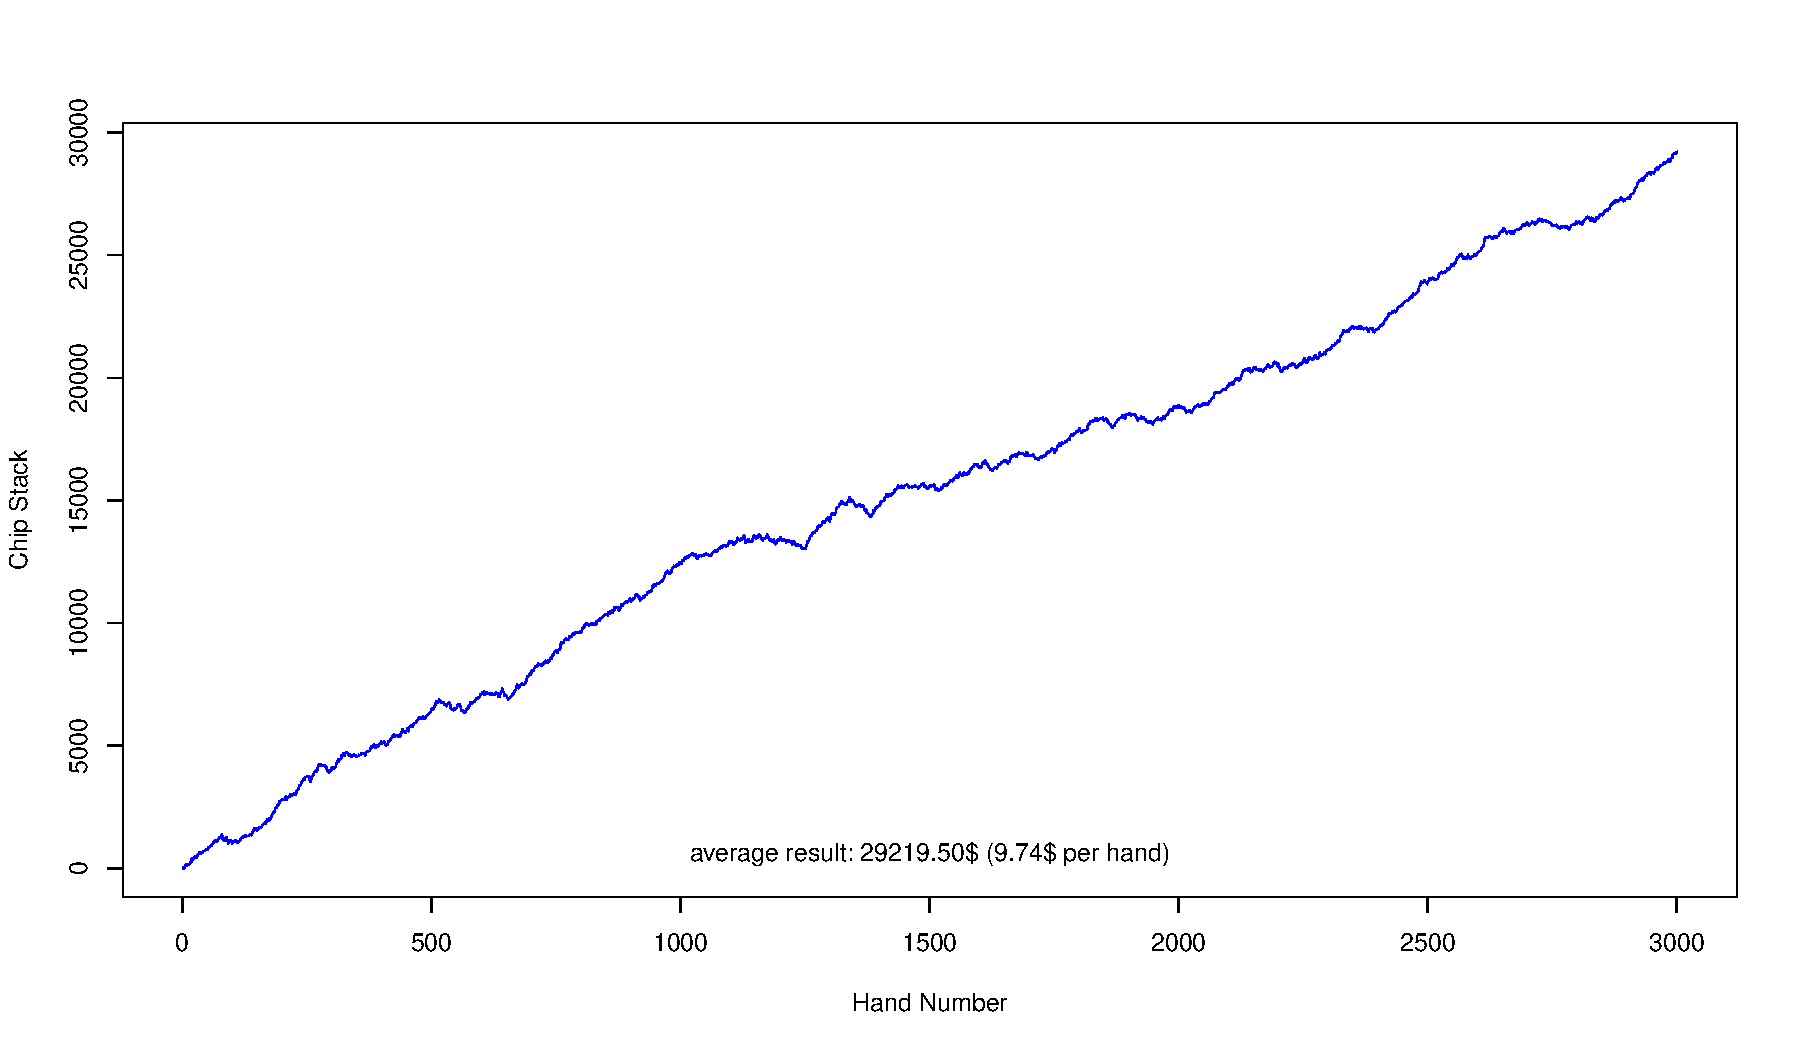
\includegraphics[width=\linewidth]{section06-implementation/figures/matchresults/AveryBot}
\caption{Matchresults: UZHoldem vs. AveryBot}
\label{fig:result-averybot}
\end{figure}

\begin{figure}[!ht]
\centering
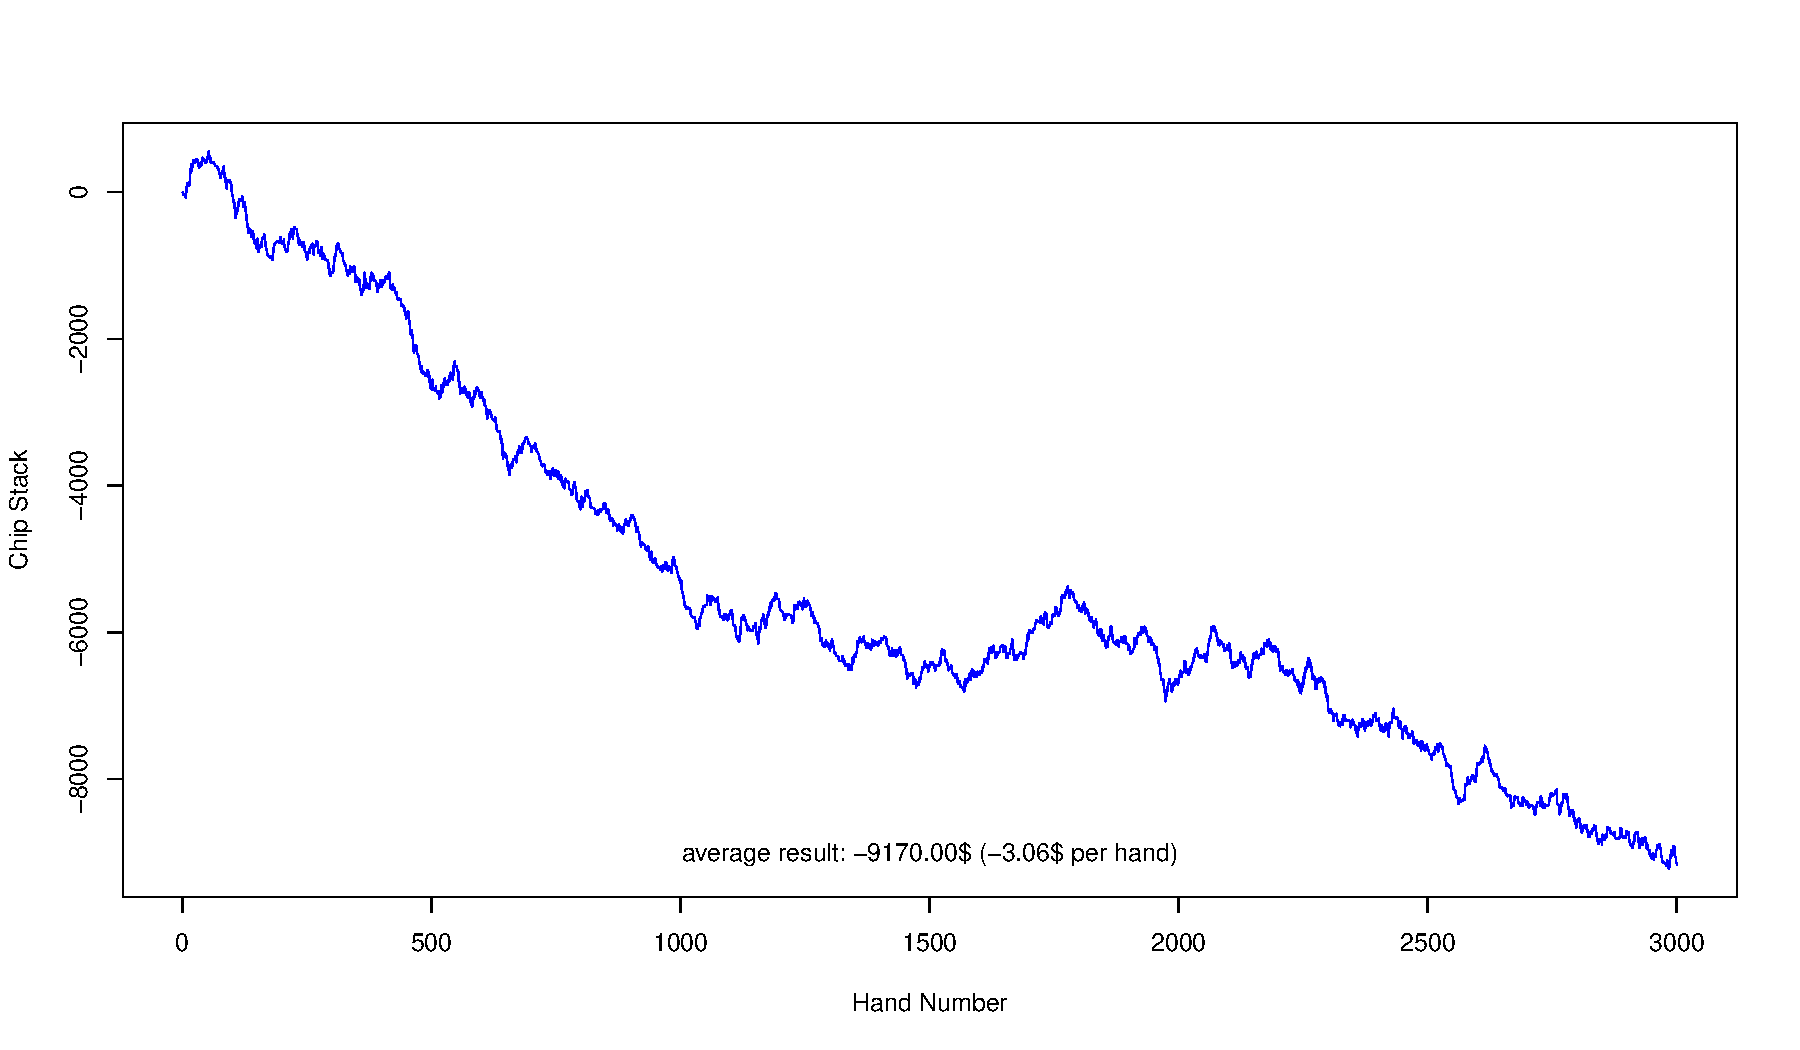
\includegraphics[width=\linewidth]{section06-implementation/figures/matchresults/XenBot}
\caption{Matchresults: UZHoldem vs. XenBot}
\label{fig:result-xenbot}
\end{figure}

\begin{figure}[!ht]
\centering
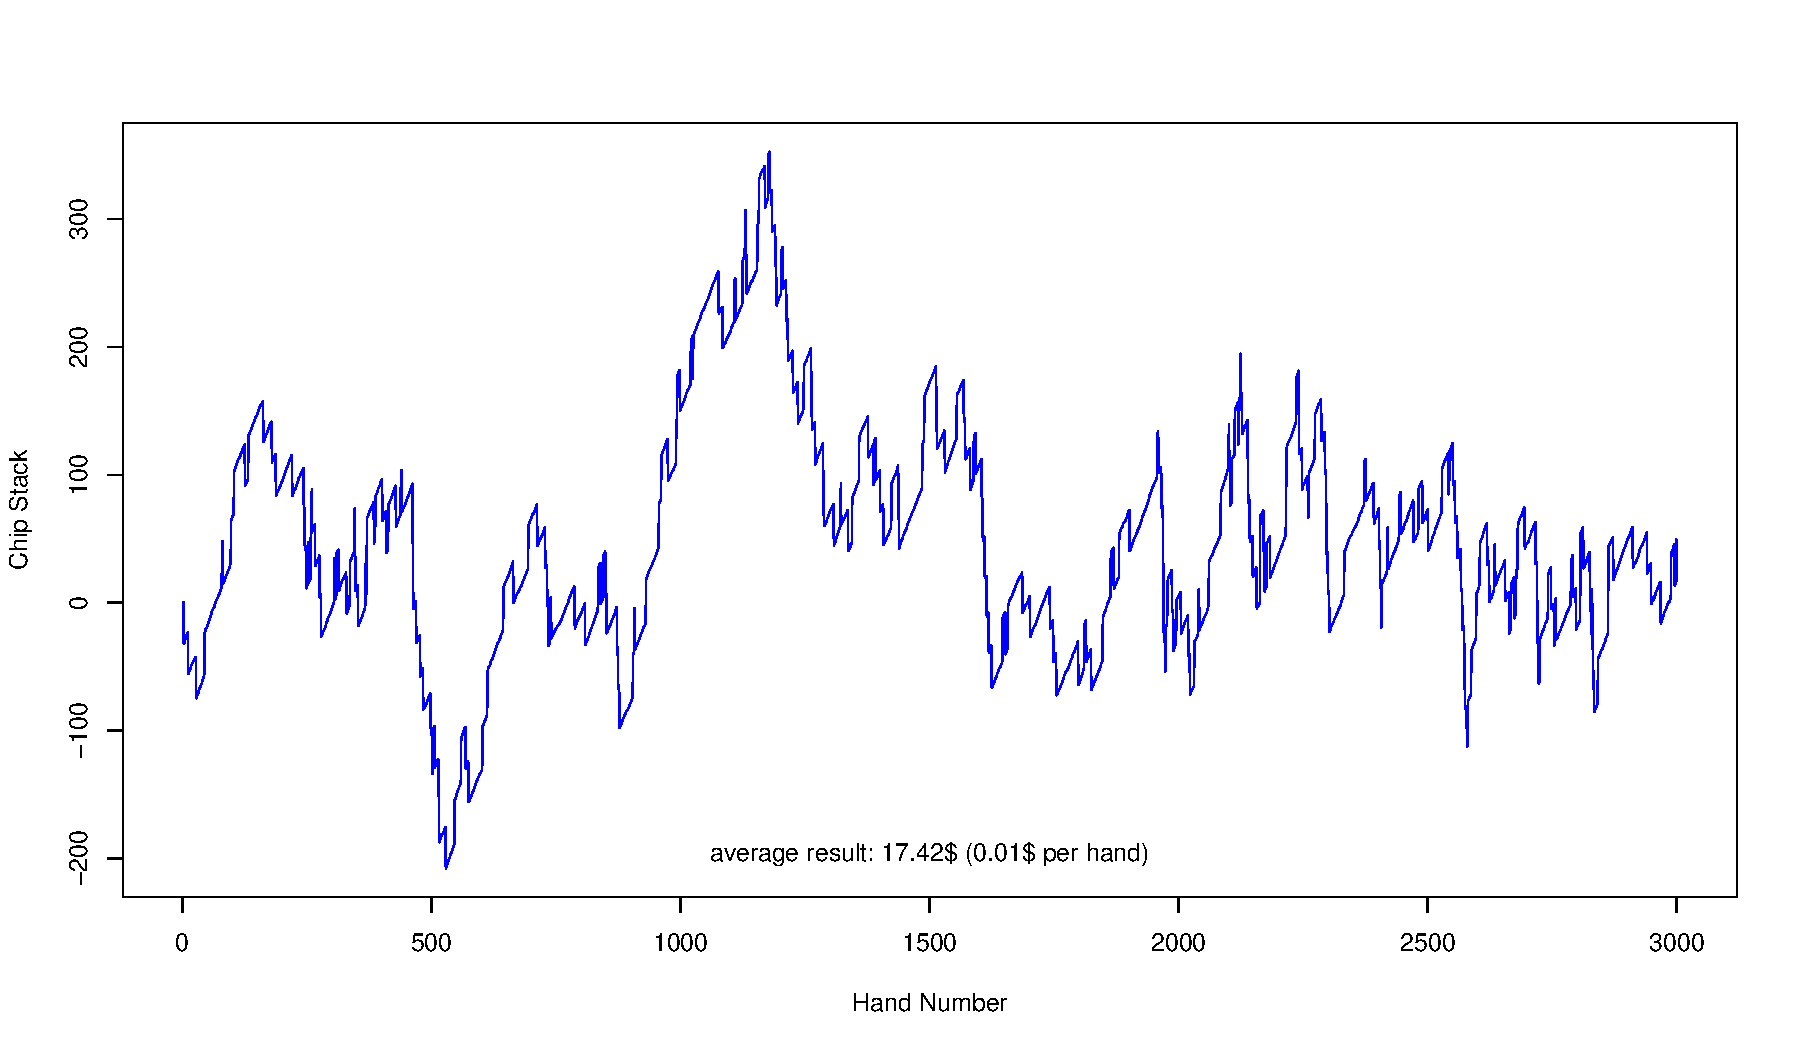
\includegraphics[width=\linewidth]{section06-implementation/figures/matchresults/JamBot}
\caption{Matchresults: UZHoldem vs. JamBot}
\label{fig:result-jambot}
\end{figure}

\begin{figure}[!ht]
\centering
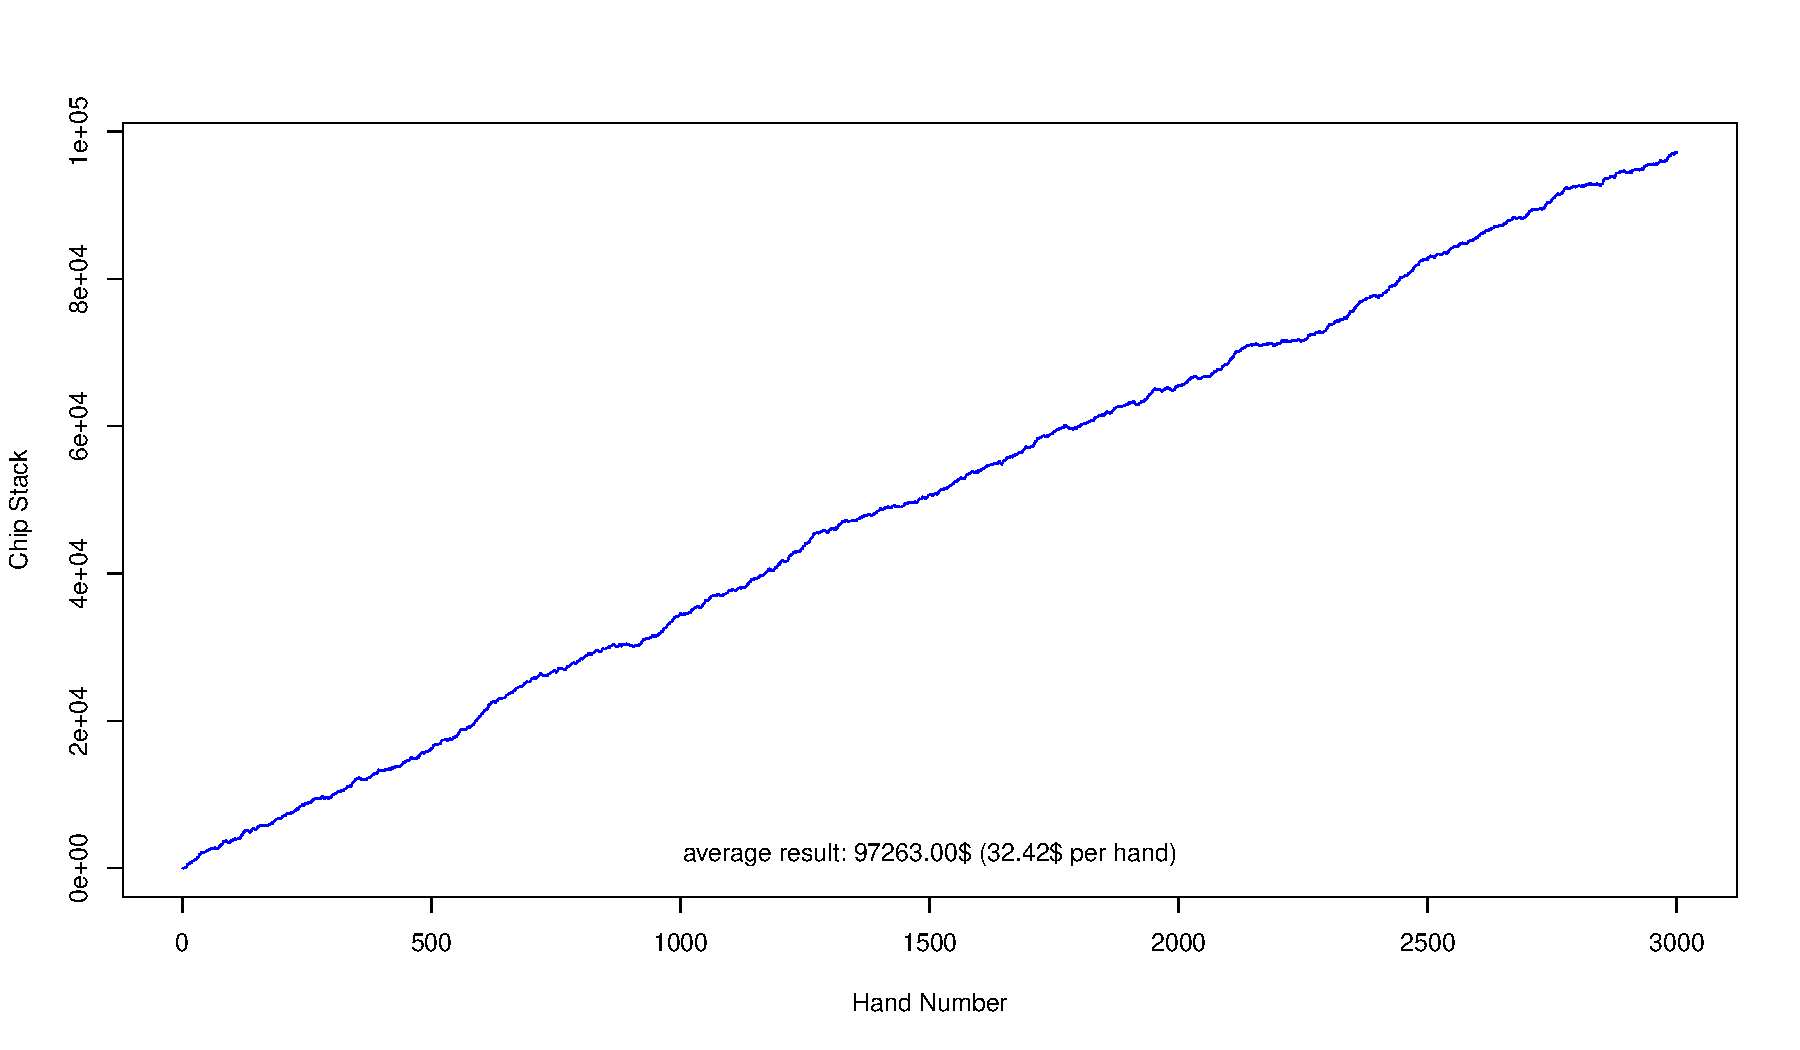
\includegraphics[width=\linewidth]{section06-implementation/figures/matchresults/Random1}
\caption{Matchresults: UZHoldem vs. Random}
\label{fig:result-random}
\end{figure}

\begin{figure}[!ht]
\centering
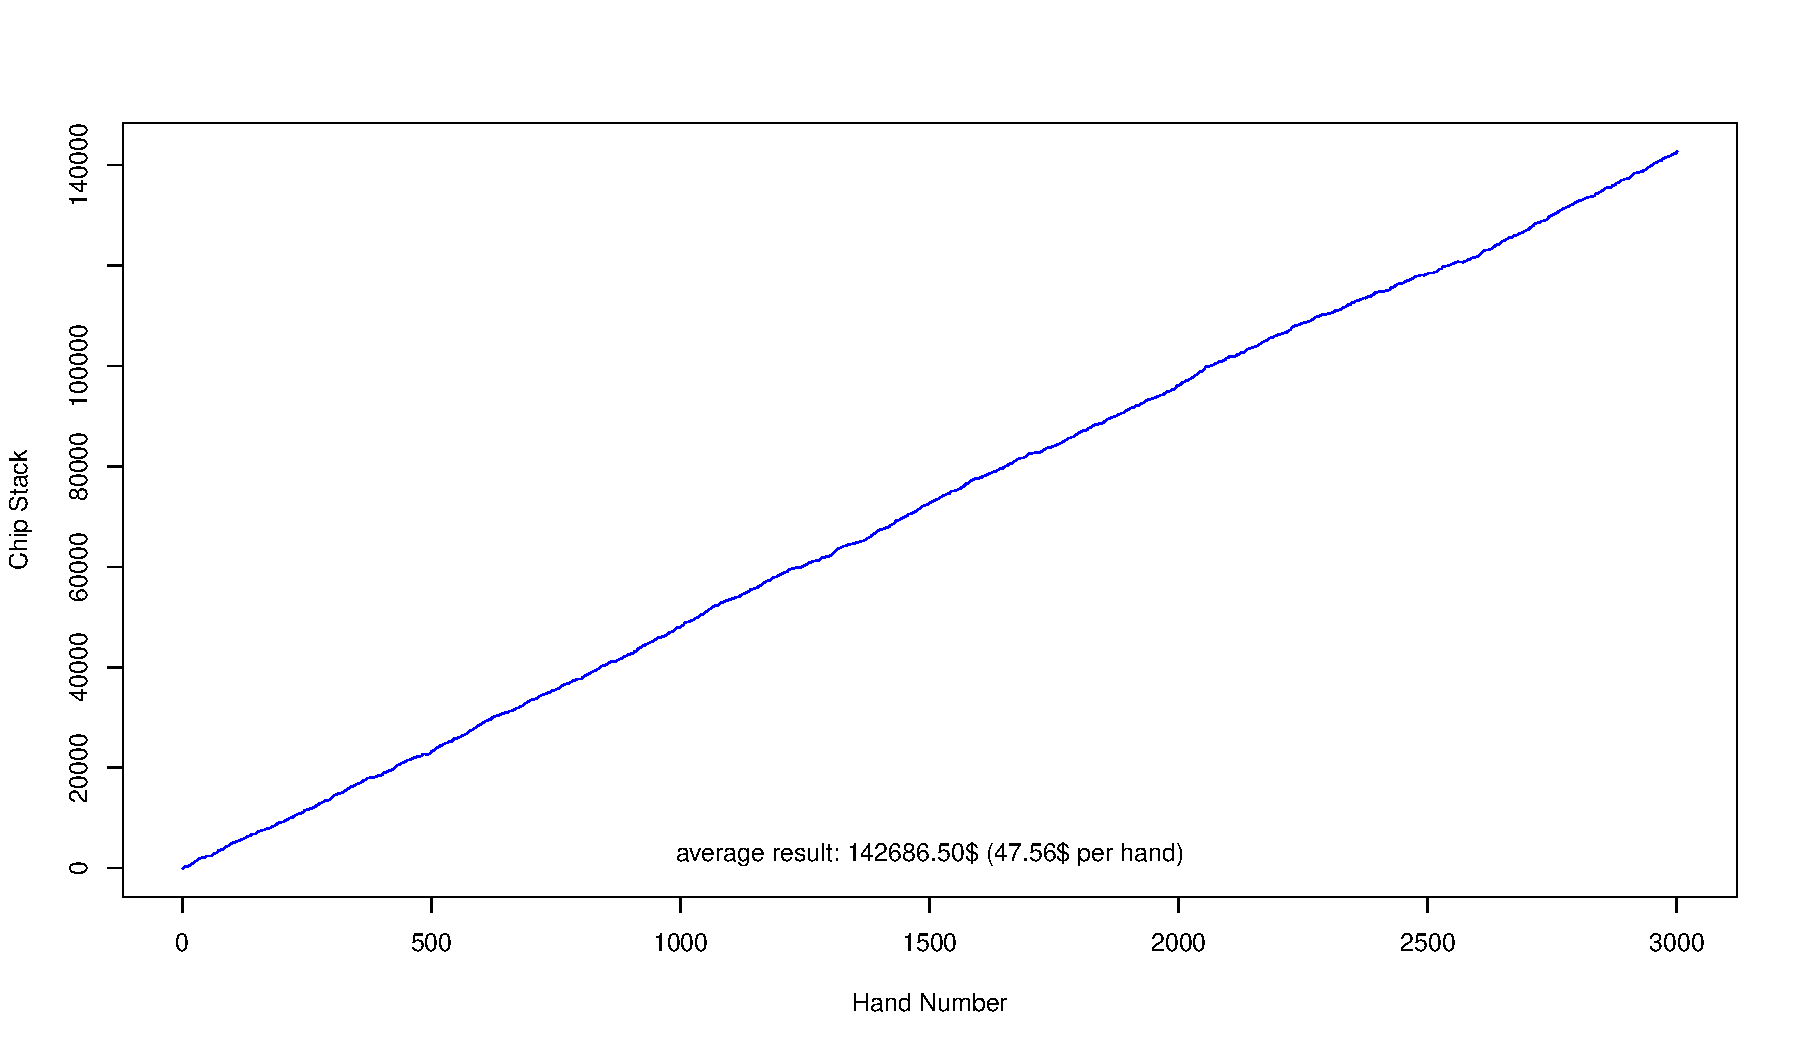
\includegraphics[width=\linewidth]{section06-implementation/figures/matchresults/AlwaysCall}
\caption{Matchresults: UZHoldem vs. AlwaysCall}
\label{fig:result-alwayscall}
\end{figure}



A two points stick out when investigating these graphs:

\begin{itemize}
	\item Even though a seemly large amount of hands were played, the variance still remains very high. This can be seen especially good in the matches against Jambot and Xenbot. This specific strategy introduces a very large variation, since all-in showdown occur rarely, but influence the result greatly.
	\item Unfortunately, all these graph show a pretty constant slope, without any signs of an performance improvement during the game, as one would probably expect from the adapting opponent model. 
\end{itemize}

\subsection{Results for Opponent Model}
To further investigate the second observation, I reran the opponent model benchmark over the game logs, to measure the improvement of the model during each match:

\subsubsection{Action Prediction}

\begin{figure}[ht!]\centering
\subfigure[Correct Predictions against Always Call]{
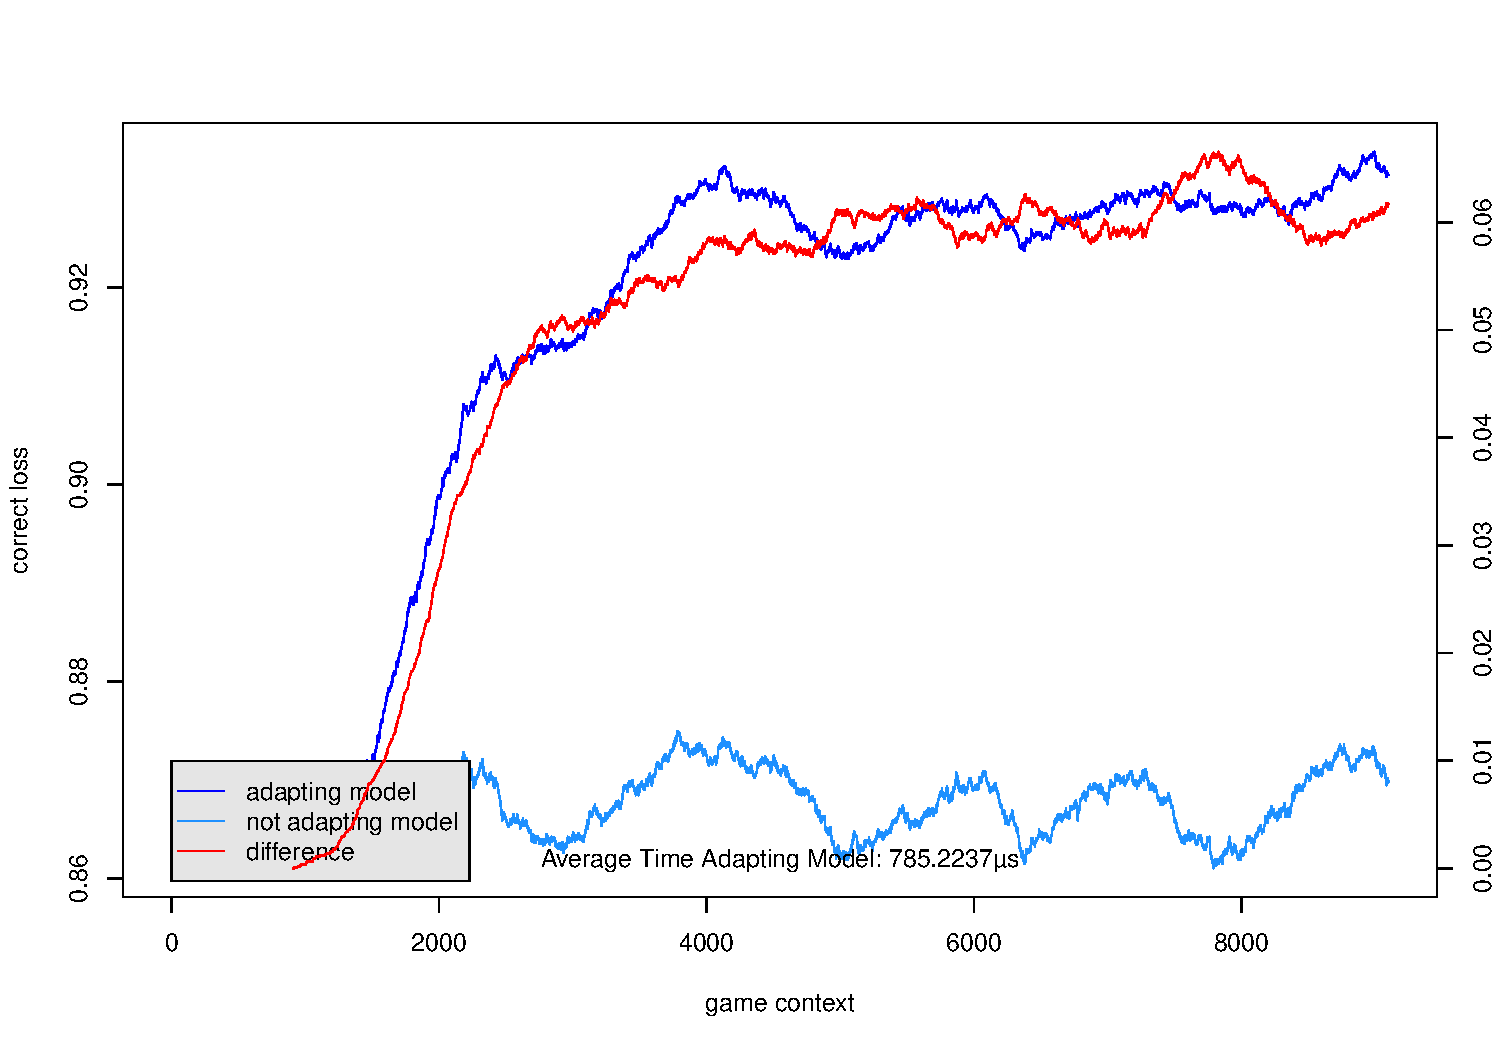
\includegraphics[scale=0.265]{section07-results/modelresults/nolimittest2-UZHoldem-AlwaysCall-action-correctly}

}
\subfigure[Quadratic Loss against Always Call]{
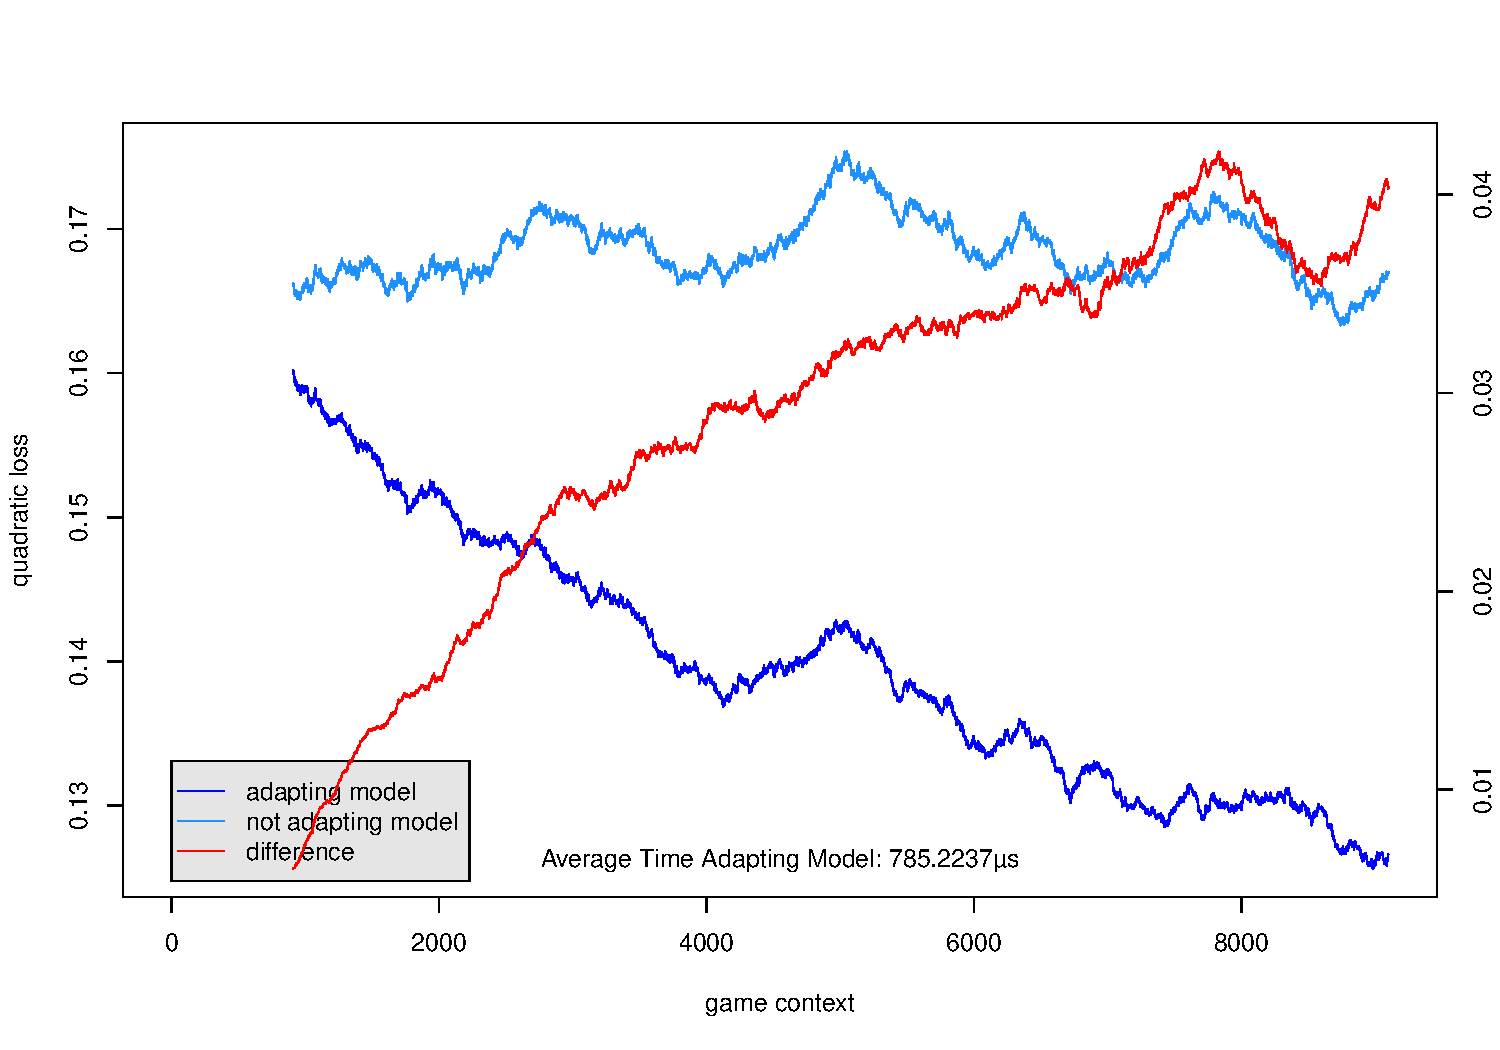
\includegraphics[scale=0.265]{section07-results/modelresults/nolimittest2-UZHoldem-AlwaysCall-action-quadratic}

}

\subfigure[Correct Predictions against Always Fold]{
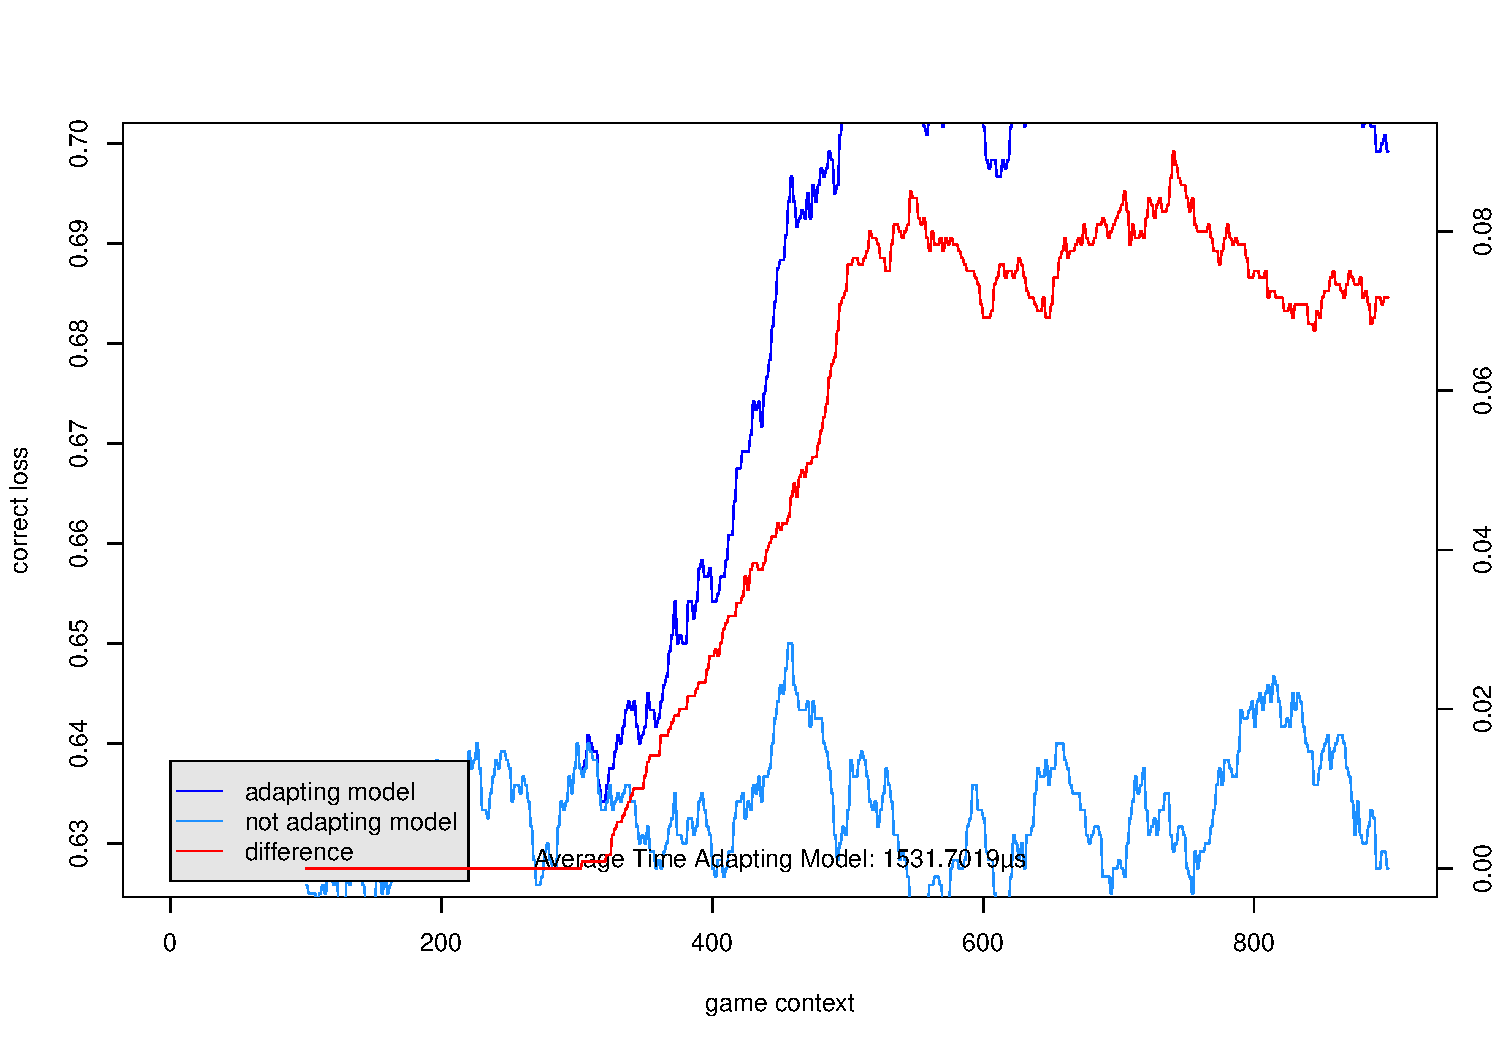
\includegraphics[scale=0.265]{section07-results/modelresults/nolimittest2-UZHoldem-AlwaysFold-action-correctly}

}
\subfigure[Quadratic Loss against Always Fold]{
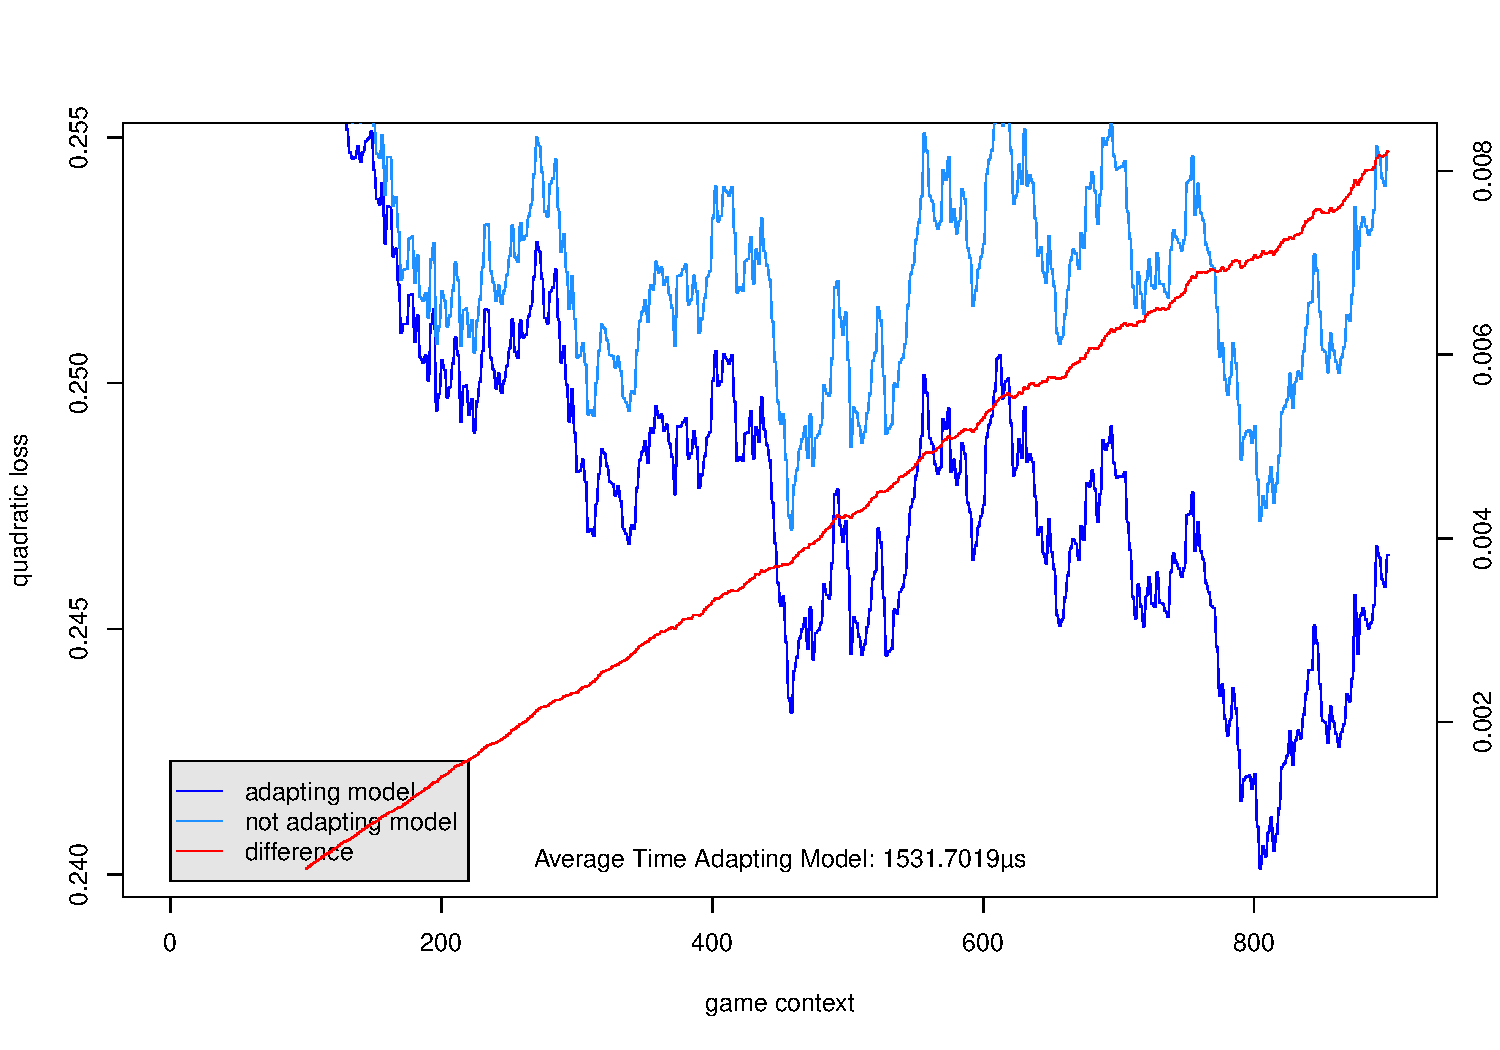
\includegraphics[scale=0.265]{section07-results/modelresults/nolimittest2-UZHoldem-AlwaysFold-action-quadratic}

}


\end{figure}

\begin{figure}[!ht]\centering
\subfigure[Correct Predictions against AveryBot]{
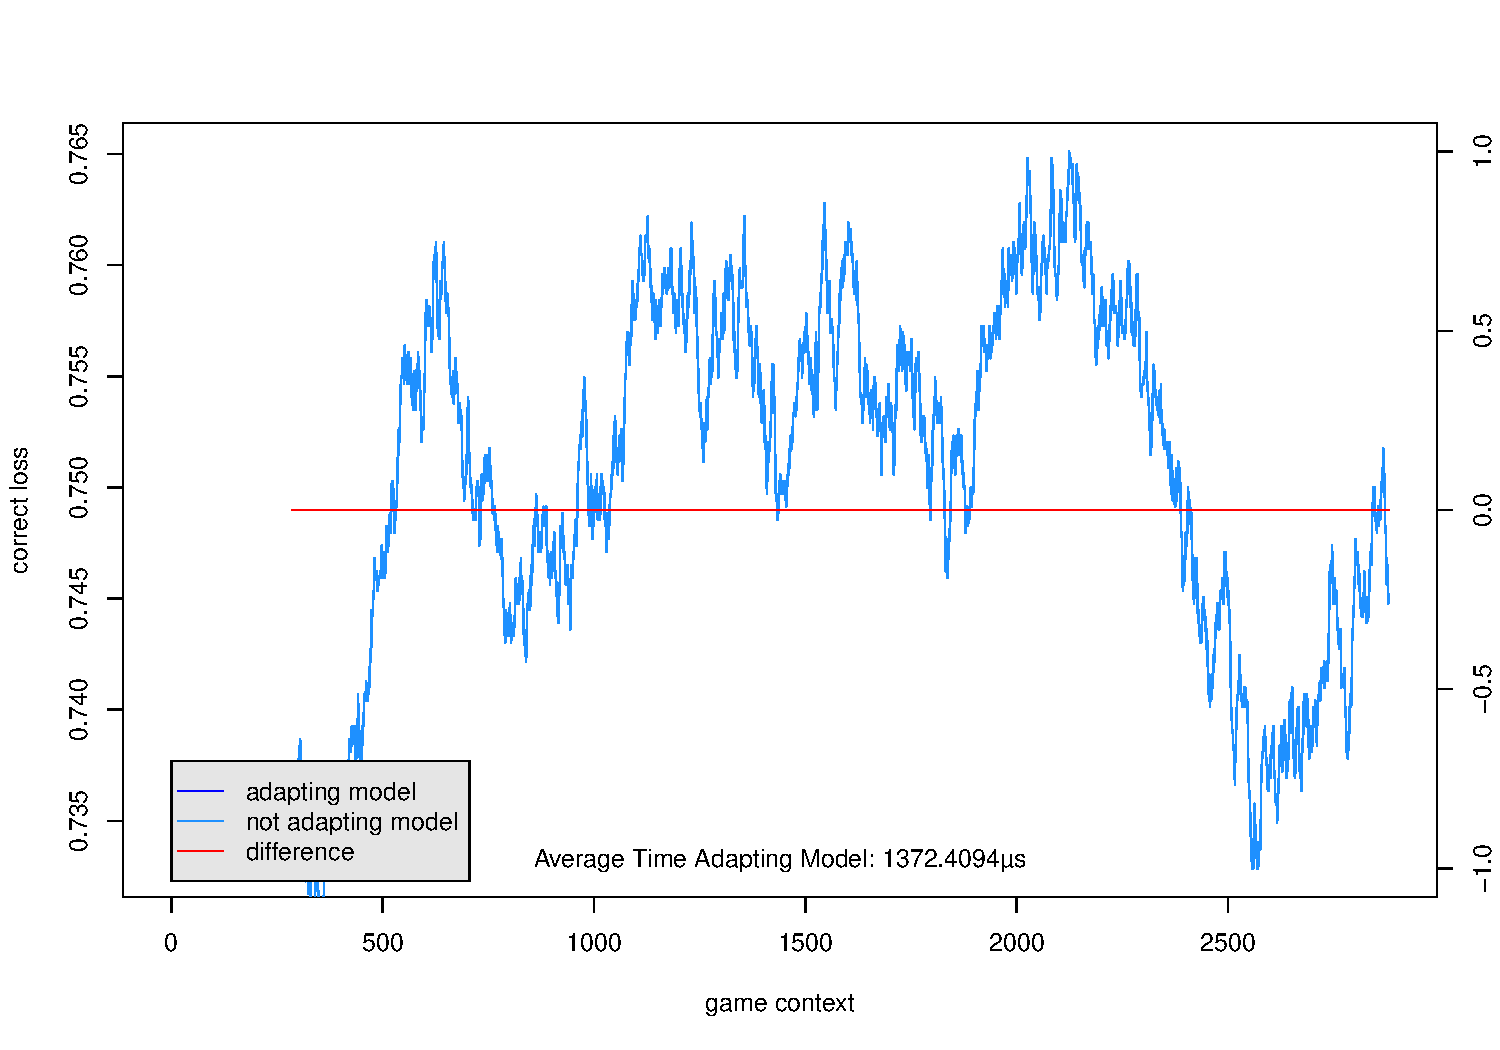
\includegraphics[scale=0.265]{section07-results/modelresults/nolimittest2-UZHoldem-AveryBot-action-correctly}

}
\subfigure[Quadratic Loss against AveryBot]{
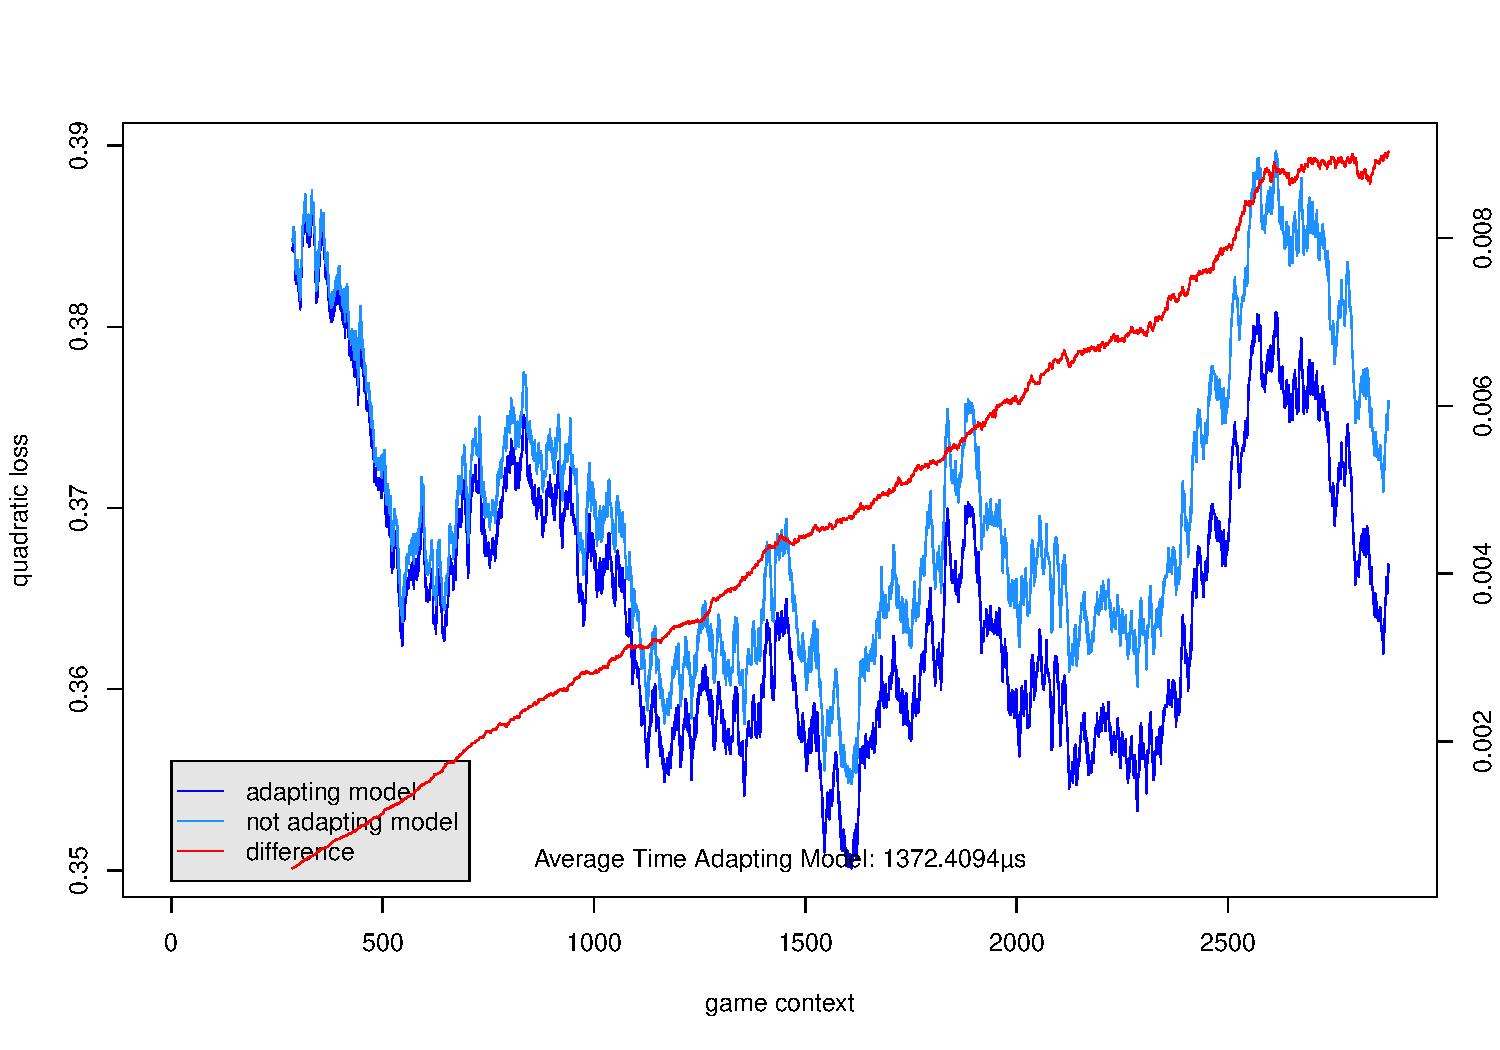
\includegraphics[scale=0.265]{section07-results/modelresults/nolimittest2-UZHoldem-AveryBot-action-quadratic}

}

\end{figure}

\begin{figure}[!ht]\centering

\subfigure[Correct Predictions against JamBot]{
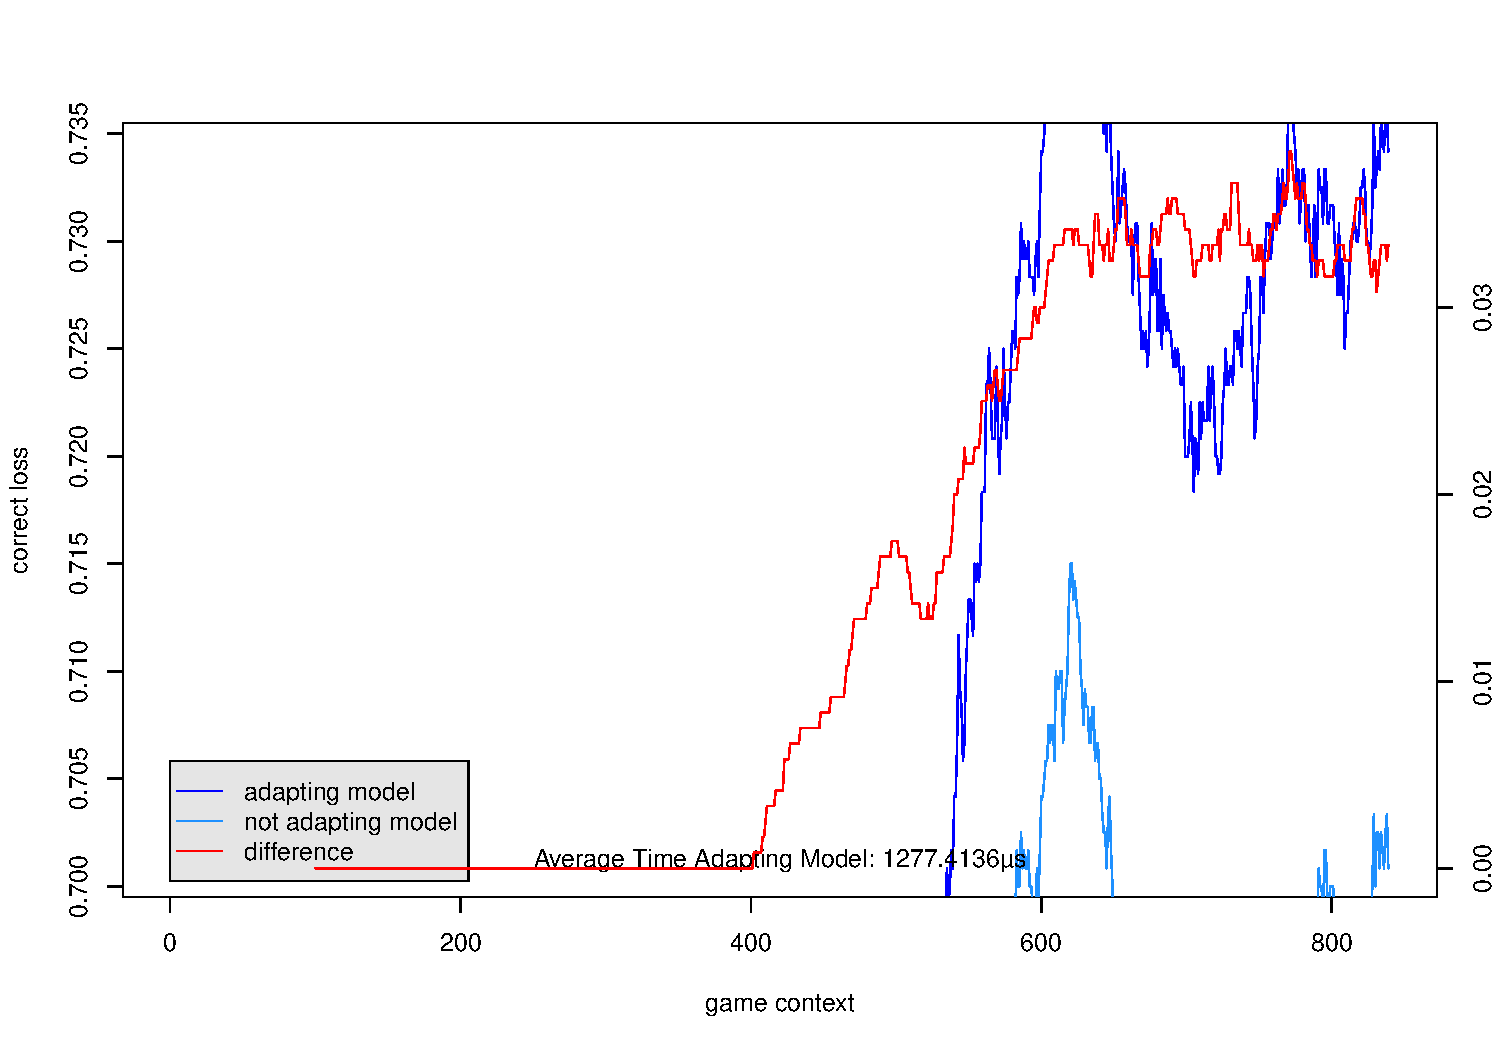
\includegraphics[scale=0.265]{section07-results/modelresults/nolimittest2-UZHoldem-JamBot-action-correctly}

}
\subfigure[Quadratic Loss against JamBot]{
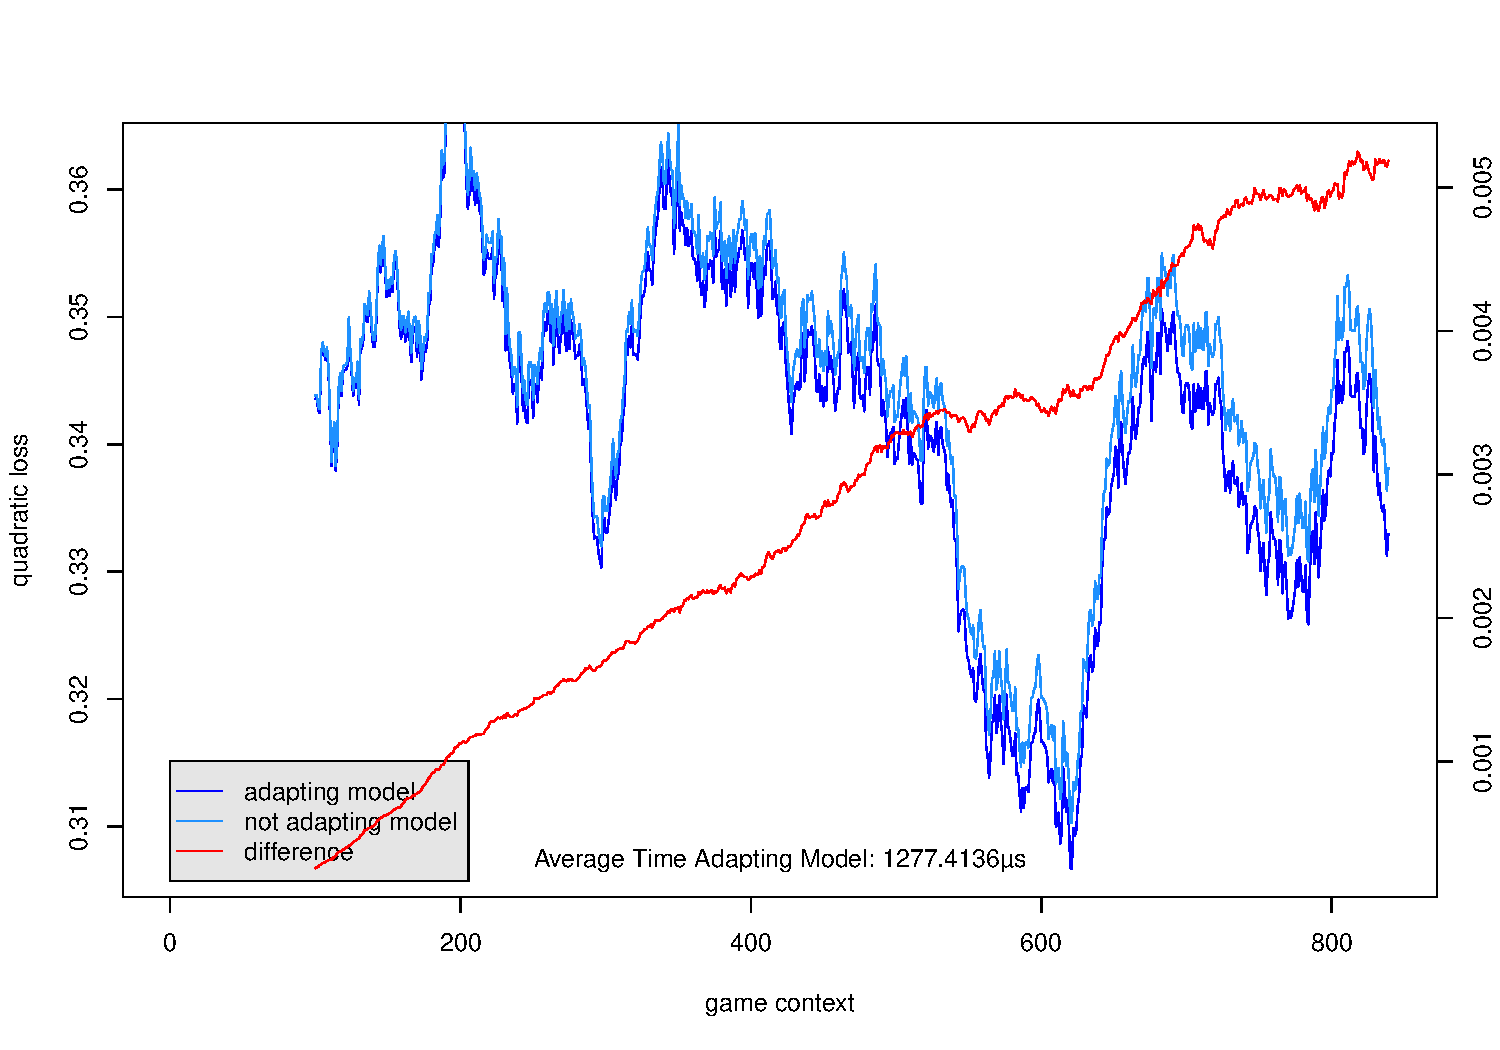
\includegraphics[scale=0.265]{section07-results/modelresults/nolimittest2-UZHoldem-JamBot-action-quadratic}

}

\subfigure[Correct Predictions against XenBot]{
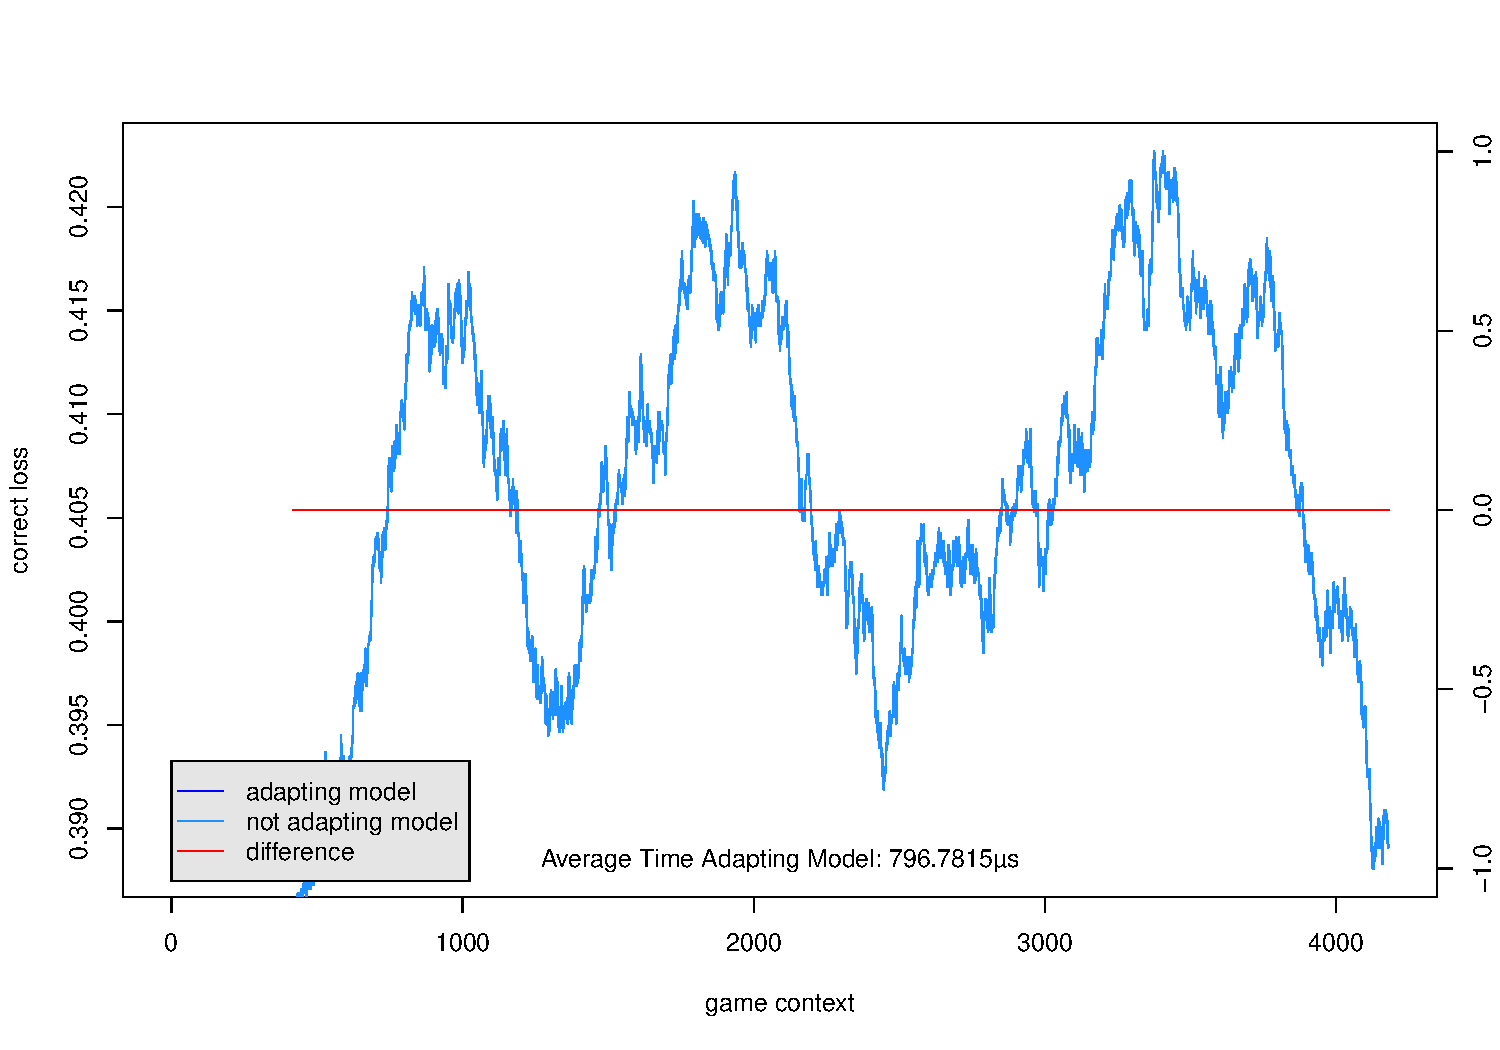
\includegraphics[scale=0.265]{section07-results/modelresults/nolimittest2-UZHoldem-XenBot-action-correctly}

}
\subfigure[Quadratic Loss against XenBot]{
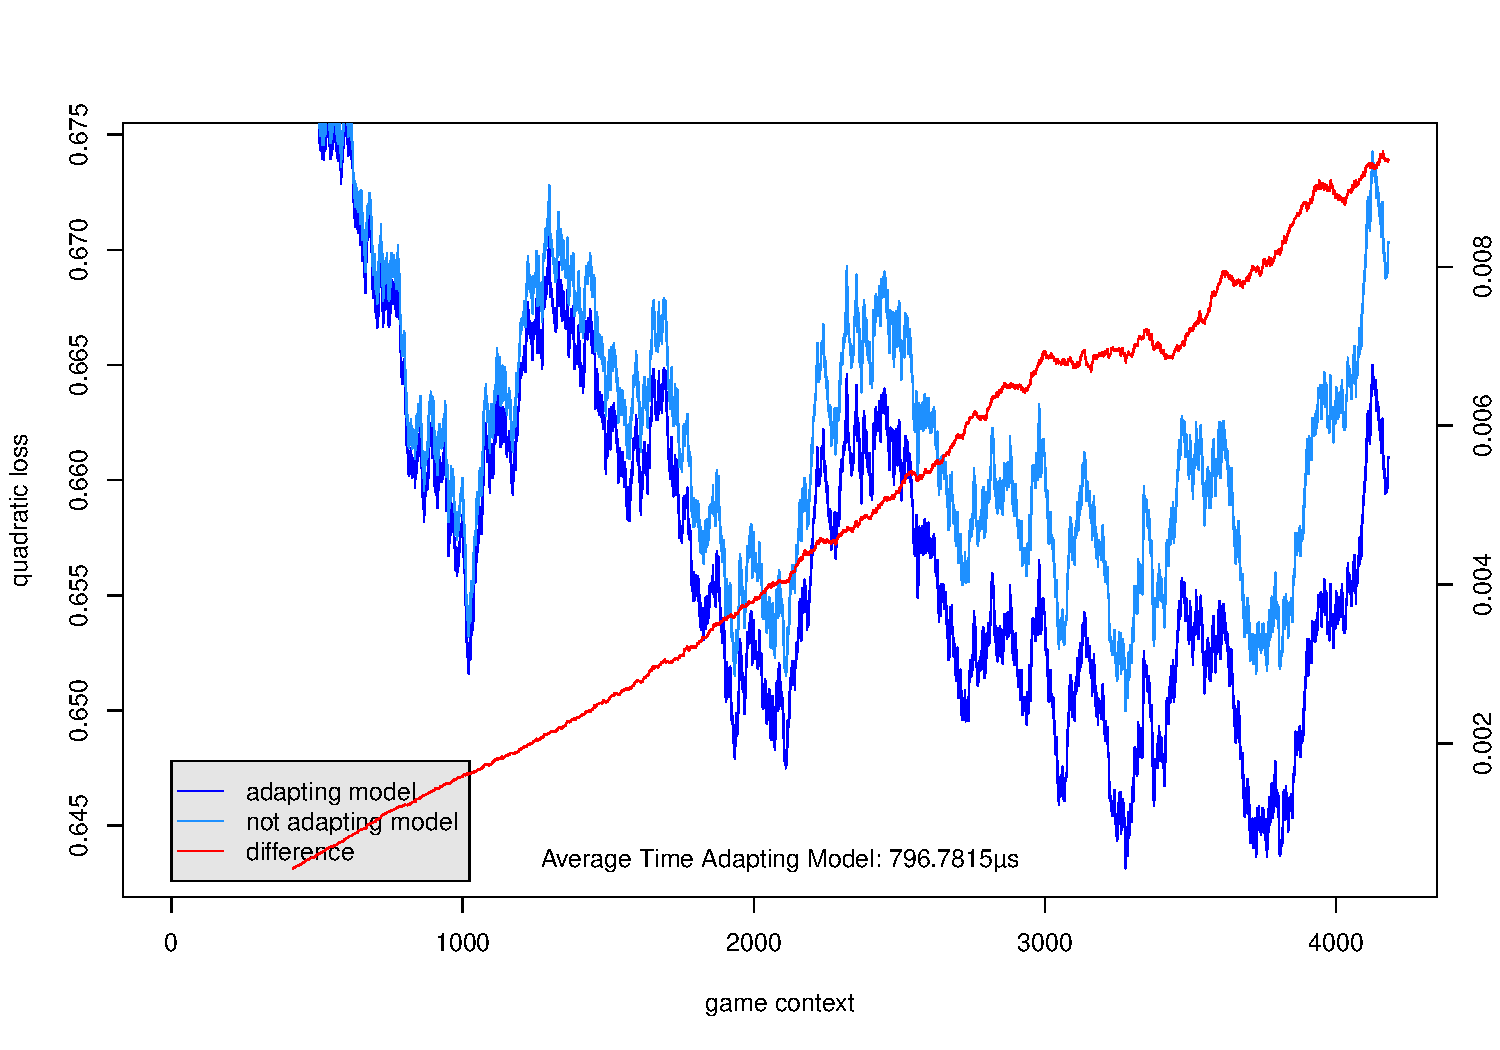
\includegraphics[scale=0.265]{section07-results/modelresults/nolimittest2-UZHoldem-XenBot-action-quadratic}

}
\caption{Action Prediction Performance}


\end{figure}

\newpage

\subsubsection{Hand Prediction}

\begin{figure}[th!]\centering
\subfigure[Mean Error against Always Call]{
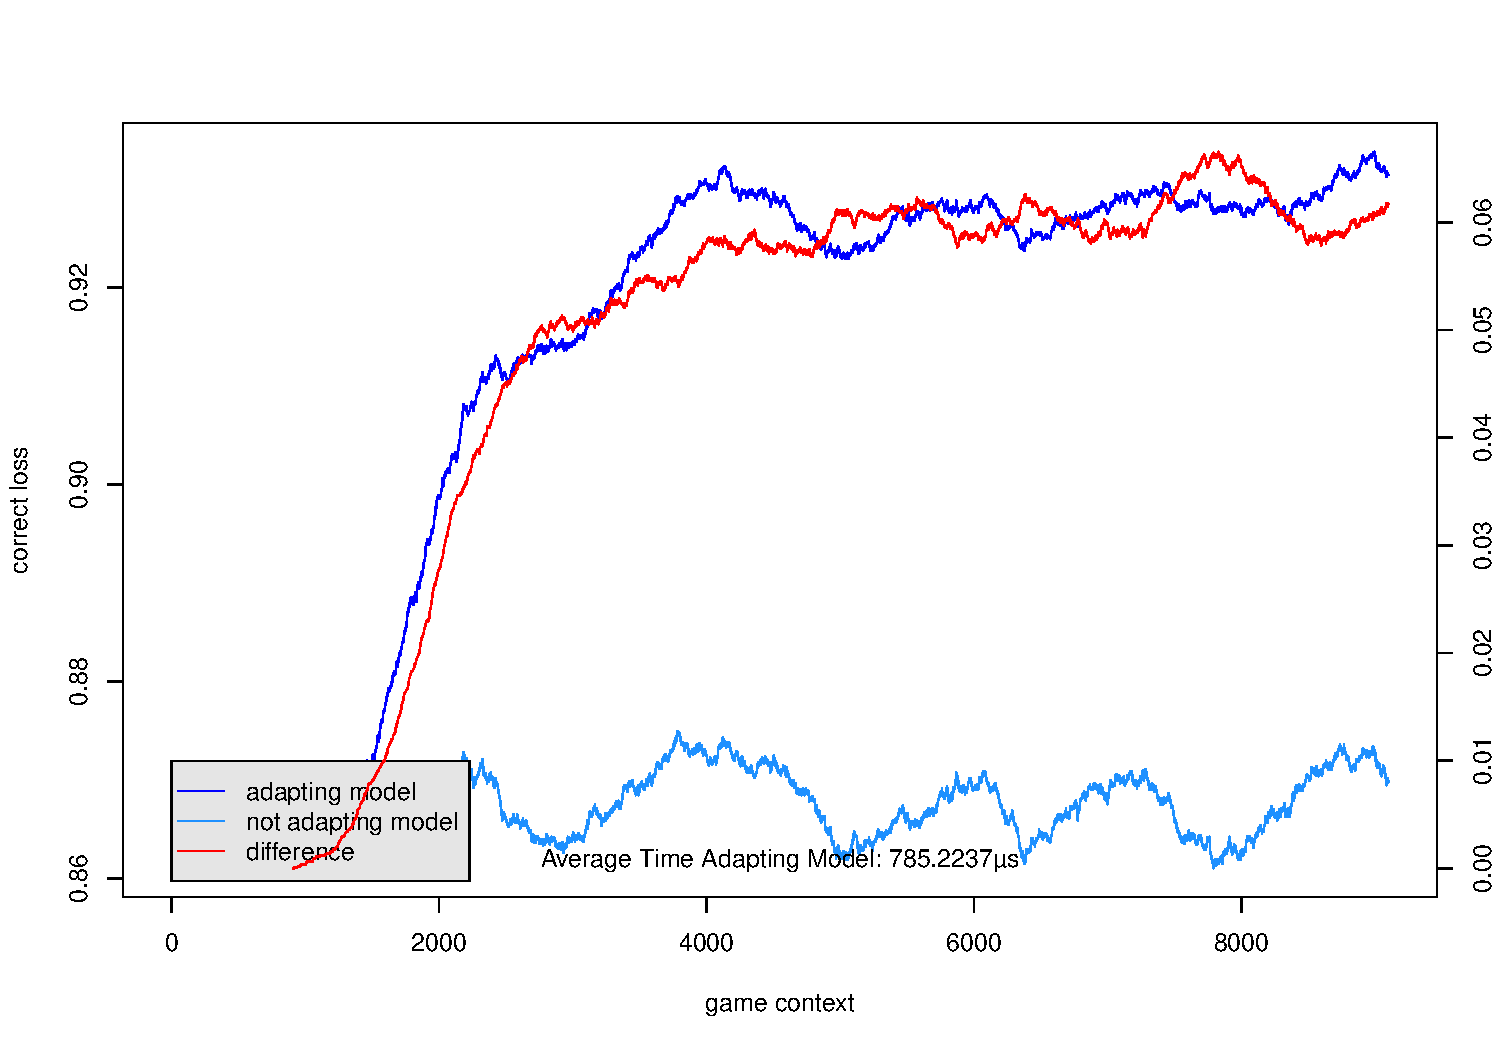
\includegraphics[scale=0.265]{section07-results/modelresults/nolimittest2-UZHoldem-AlwaysCall-action-correctly}

}
\subfigure[Quadratic Loss against Always Call]{
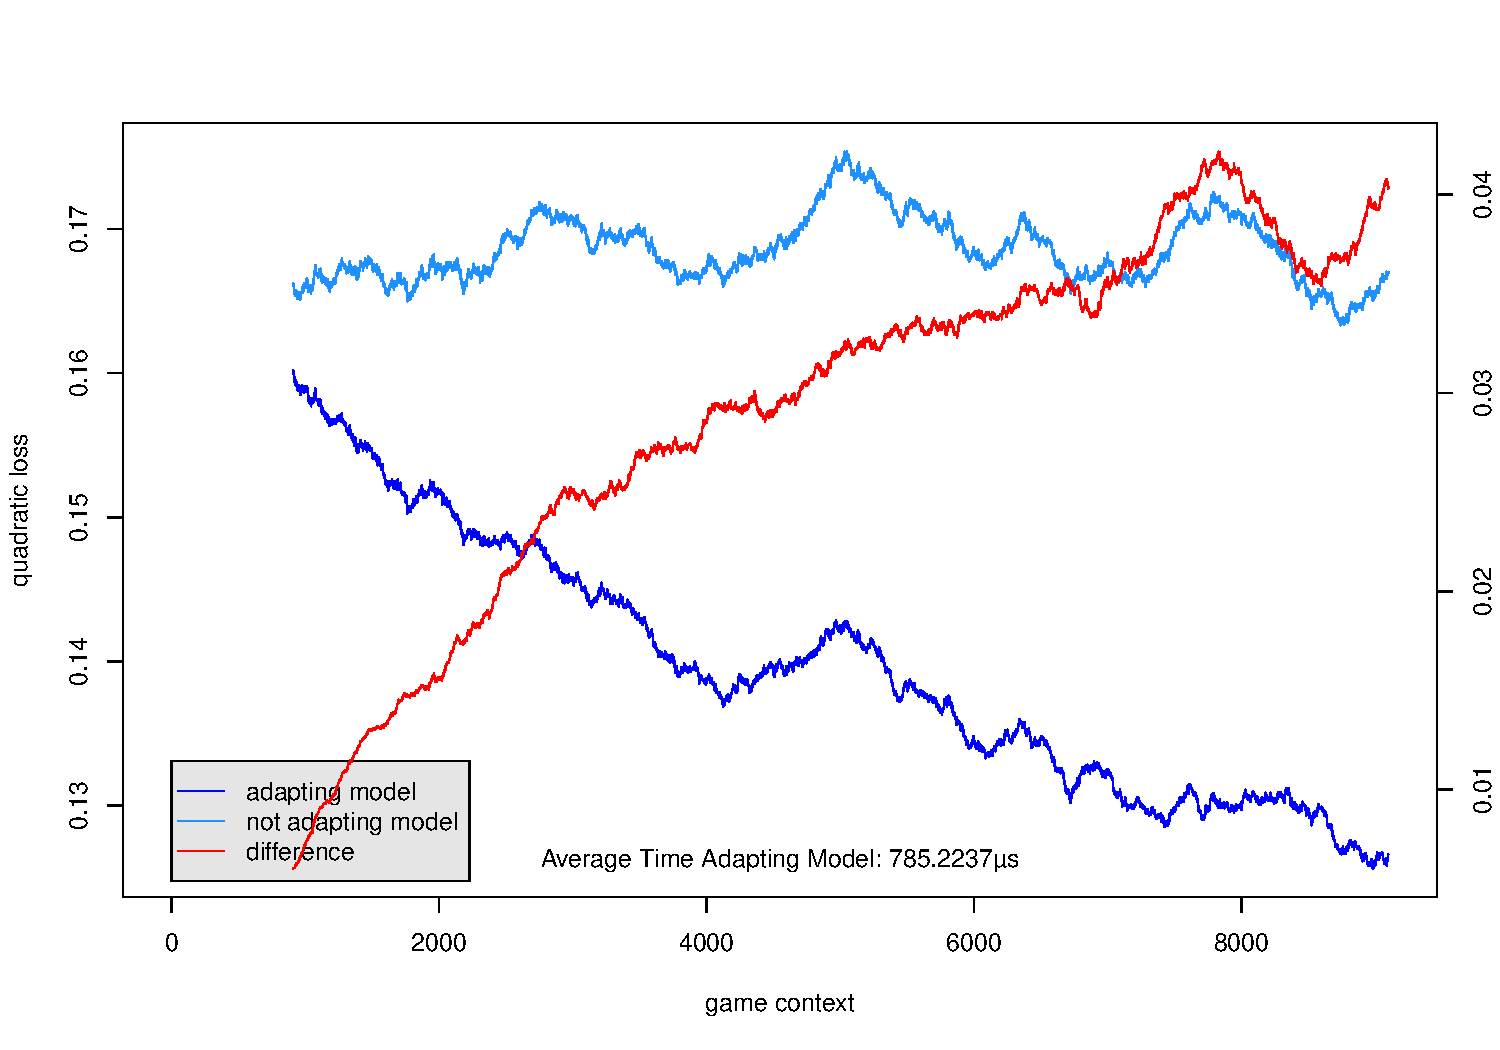
\includegraphics[scale=0.265]{section07-results/modelresults/nolimittest2-UZHoldem-AlwaysCall-action-quadratic}

}

\end{figure}

\begin{figure}[!ht]\centering


\subfigure[Mean Error against AveryBot]{
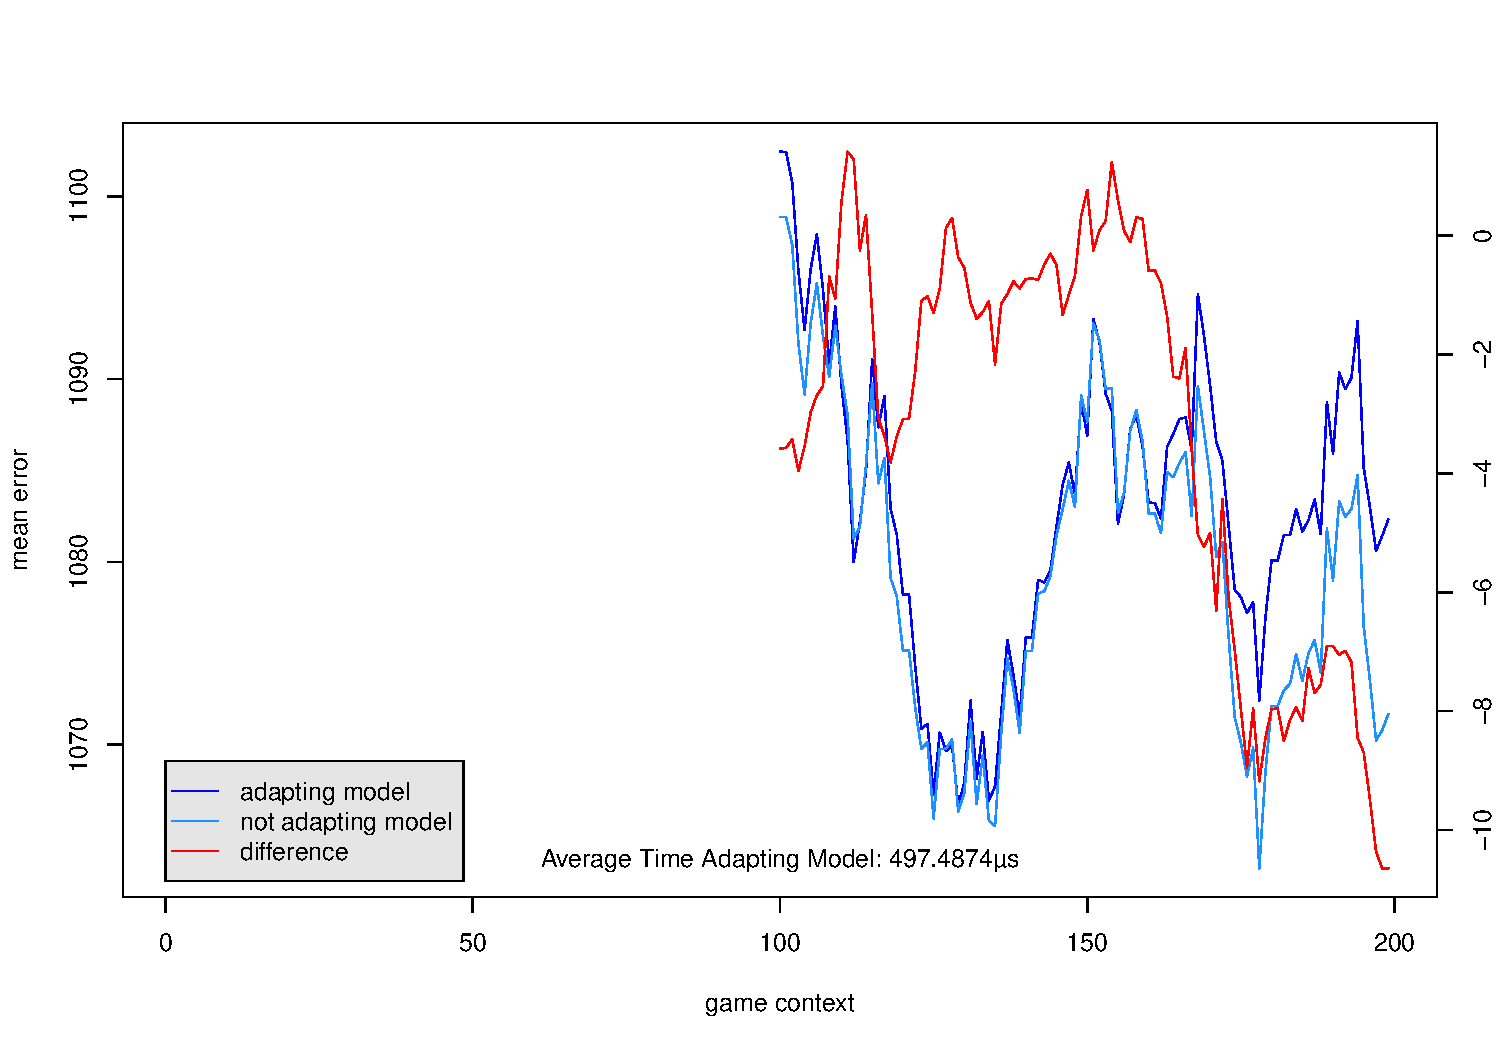
\includegraphics[scale=0.265]{section07-results/modelresults/nolimittest2-UZHoldem-AveryBot-hand-meansquared}

}
\subfigure[Quadratic Loss against AveryBot]{
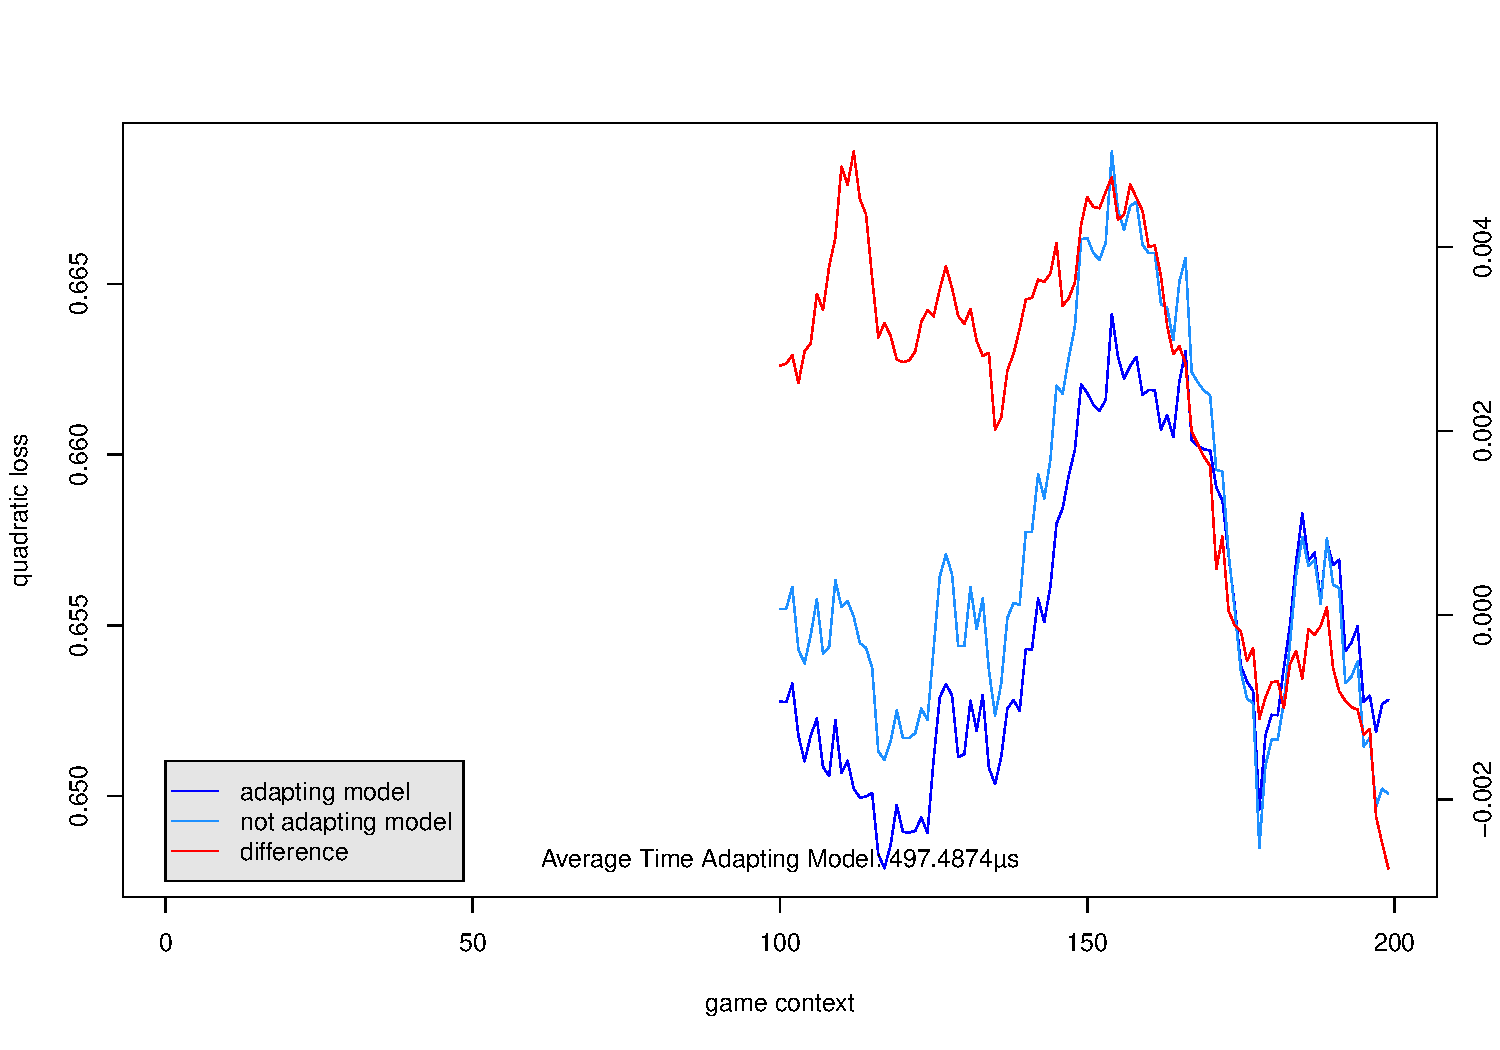
\includegraphics[scale=0.265]{section07-results/modelresults/nolimittest2-UZHoldem-AveryBot-hand-quadratic}

}


\end{figure}

\begin{figure}[!ht]\centering

\subfigure[Mean Error against XenBot]{
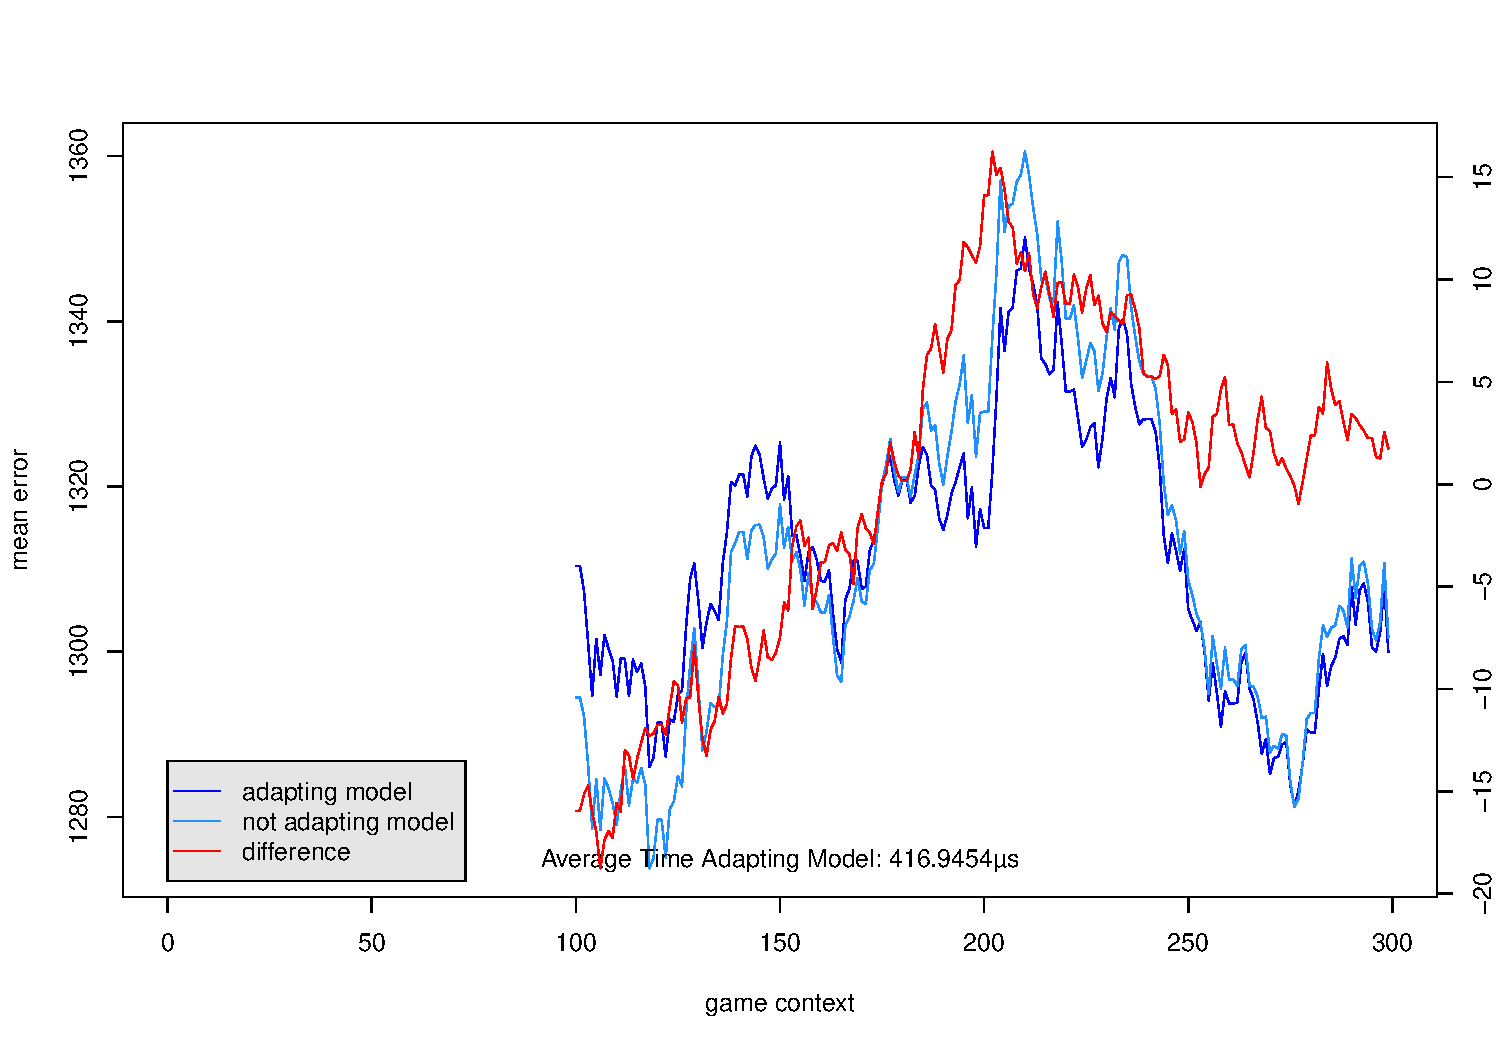
\includegraphics[scale=0.265]{section07-results/modelresults/nolimittest2-UZHoldem-XenBot-hand-meansquared}

}
\subfigure[Quadratic Loss against XenBot]{
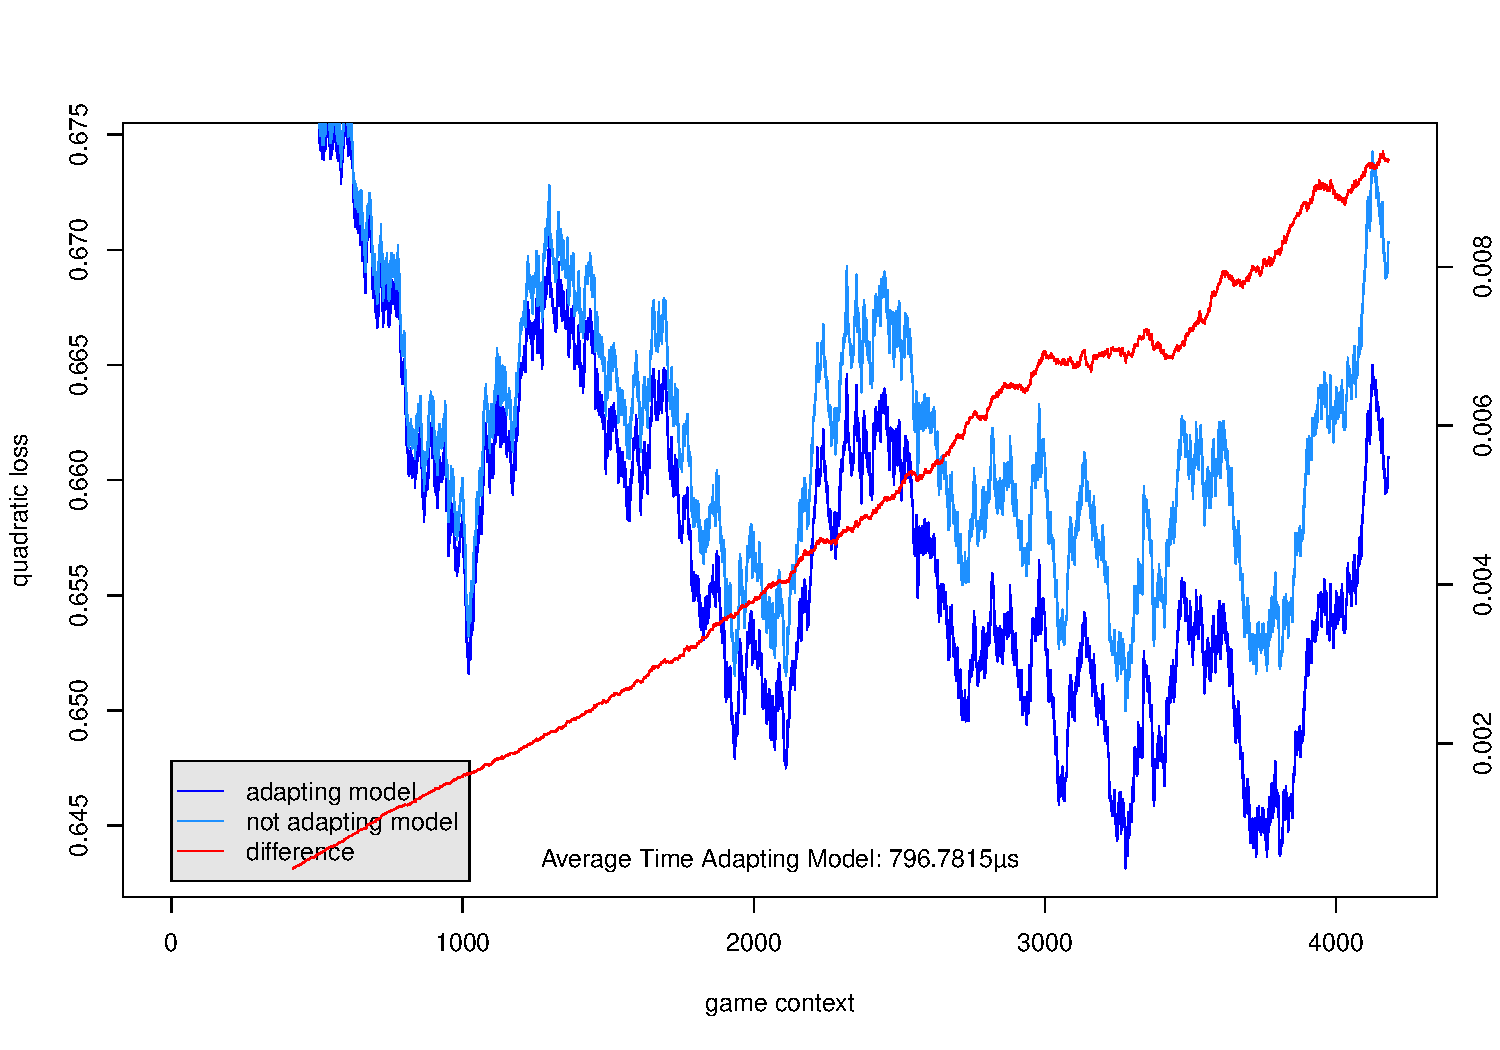
\includegraphics[scale=0.265]{section07-results/modelresults/nolimittest2-UZHoldem-XenBot-action-quadratic}

}
\caption{Hand Prediction Performance}


\end{figure}

\newpage
\section{Insights from playing against humans}

To better judge the resulting program in regard to its style of play, I also conducted a round of hands against a human player. This informal experiment should provide a subjective view on how a opponent unaware of the underlining algorithm perceives the resulting play style. To do this, the bot was added to \textit{Poker Academy}, which provided the graphical user interface for the interface. The manual in the appendix explains the necessary steps to play UZHoldem in \textit{Poker Academy}.

\subsection{Pre-Flop Play}

Little surprising, the pre-flop strategy was perceived as very week and transparent. While the algorithm is very defensive versus all-in moves by the opponent, it still re-raises minimal-raises all the way down to a all-in. But if the opponent raises, the program re-raises, and if the player then goes all-in, the program decides to fold. 

\subsection{Post-Flop Play}

Playing after the flop has been dealt was perceived much stronger. While still being somewhat strange, and riddled with exploitable weaknesses, its moves generally make sense. Some observed weaknesses include:

\begin{itemize}
\item Draws are often played extremely aggressive, even re-raising raises.
\item Pairs on the flop are often played very weak, but then suddenly very aggressive on the river, sometimes going all-in, even though the hand didn't improve at all.
\item The hight of a pair seems to not have much of an effect. This results in a overly strong play of weak bottom pairs, calling or raising them all the way to a showdown.
\item The algorithms seems to underestimates the chance of the opponent folding to an all-in move. All-in bets on the flop result in a fold in the vast majority of cases. Still, UZHoldem often bets all-in having the highest pair, obviously assuming this to be a bet that might extract the most money from the opponent. This results in the opponent only calling with absolute winning hands, and folding everything else, resulting in only very small winning but large losses.
\item Generally, the line of actions during a hand is often perceived as random. UZHoldem might bet on the flop, then check on the turn, bet on the river but then fold when faced a raise. Other strange lines include checking on the flop, then calling on the turn and betting all-in on the river as a bluff.
\end{itemize}

Overall, the bot has shown mix performance, which might be comparable to a novice of the game, but unable to derange a more experienced player.